\documentclass[conference]{IEEEtran}
\IEEEoverridecommandlockouts
% The preceding line is only needed to identify funding in the first footnote. If that is unneeded, please comment it out.
\usepackage{cite}
\usepackage{hyperref}
\usepackage{amsmath,amssymb,amsfonts}
\usepackage{algorithmic}
\usepackage{graphicx}
\usepackage{textcomp}
\usepackage{xcolor}
\usepackage{float} 
\usepackage{graphicx}
\usepackage{placeins}
\usepackage{hyperref}
\usepackage{float}
\def\BibTeX{{\rm B\kern-.05em{\sc i\kern-.025em b}\kern-.08em
    T\kern-.1667em\lower.7ex\hbox{E}\kern-.125emX}}

    
\begin{document}

%%%%%%---------------------------------cover page
\begin{titlepage}
    \thispagestyle{empty} % removes header/footer on this page
    \centering
    \vspace*{0cm}
    
\begin{figure}[htbp]
    \centering
    
\includegraphics[width=0.4\linewidth]{./figs/just_logo.JPG}
    %\caption{System architecture of the proposed Arabic Sign Language recognition model.}
    \label{fig:logo}
\end{figure}

    
   % {\LARGE %\textbf{Project Proposal}}\\[1.2cm]}
    {\Huge \textbf{Early Neonatal Sepsis Prediction Using Patient-Aware Time-Series Modeling with Clinical Realism }}\\[1.5cm]
    {\large Final Project Report Submitted to \\
The Department of Computer Science \\
Faculty of Computer and Information Technology \\
Jordan University of Science and Technology \\

In Partial Fulfillment of the Requirements for the Degree of Bachelors of Science in Computer Science}\\

\vspace*{1cm}


    {\Large Prepared by:}\\[0.4cm]
    {\Large Malik Jallal [163106]\\
    {\Large Lujain To'ma [162210]\\}
    {\Large Areen Alakaleek  [164150]\\}
    {\Large Motasem Alwedyan  [164948]\\}
    
 \vspace*{1cm}  
    
    { \Large Supervisor: \\}
    {\Large  Ahmad Alzubi }\\[2cm]
    
    {\large January 2026}\\[3cm]
    
    \vfill
\end{titlepage}
%%%%---------------end of comver page -----------------
\newpage
\begin{figure}[htbp]
    \centering
    
\includegraphics[width=1\textwidth]{./figs/arabic_tanazol.JPG}
    %\caption{System architecture of the proposed Arabic Sign Language recognition model.}
    \label{fig:tanazol }
\end{figure}



%%%%%--------------------------


\title{Early Neonatal Sepsis Prediction Using Patient-Aware Time-Series Modeling with Clinical Realism  \\
%{\footnotesize \textsuperscript{*}Note: Sub-titles are not captured %in Xplore and
%should not be used}
\thanks{Identify applicable funding agency here. If none, delete this.}
}
\usepackage{hyperref} % تأكدي إنها موجودة في الـ preamble

\author{
Malik Jallal\textsuperscript{1},
Lujain To’ma\textsuperscript{1},
Areen Al-Akaleek\textsuperscript{1},
Motasem Alwedyan\textsuperscript{1},
Ahmad Alzubi\textsuperscript{2}\\[0.3em]

\textsuperscript{1}\textit{Department of Computer Science, Artificial Intelligence}\\
\textit{Jordan University of Science and Technology}\\
Irbid, Jordan\\
\textsuperscript{1}\href{mailto:mtjalal22@cit.just.edu.jo}{mtjalal22@cit.just.edu.jo},
\href{mailto:lytoma22@cit.just.edu.jo}{lytoma22@cit.just.edu.jo},
\href{mailto:aaalakaleek22@cit.just.edu.jo}{aaalakaleek22@cit.just.edu.jo}
\href{mailto:mbalwedyan22@cit.just.edu.jo}{mbalwedyan22@cit.just.edu.jo},
\\[0.3em]


\textsuperscript{2}\href{mailto:agalzubi@just.edu.jo}{agalzubi@just.edu.jo}
}



\maketitle

\begin{abstract}
Neonatal sepsis remains a critical cause of morbidity and mortality among newborns, particularly in Neonatal Intensive Care Units (NICUs), where early detection is essential for improving clinical outcomes. Despite the growing use of machine learning and deep learning techniques for sepsis prediction, many existing approaches suffer from methodological limitations, including patient-level data leakage, unrealistic evaluation protocols, and limited clinical applicability.

In this work, we propose a clinically grounded, patient-aware multi-model learning framework for early neonatal sepsis prediction using multivariate physiological time-series data. The proposed approach integrates classical machine learning models, including XGBoost, with deep learning architectures such as LSTM, alongside an optimized ensemble model to improve robustness and generalization.

To ensure clinical realism, the framework incorporates strict patient-level data splitting, a 24-hour forecasting formulation, and a comprehensive preprocessing pipeline addressing data imbalance and physiological plausibility. Additionally, a dedicated clinical alerting mechanism is introduced, combining exponential moving average (EMA) smoothing, k-of-n detection, and a refractory period to reduce false alarms and enhance practical deployment.

Extensive experiments demonstrate that the proposed framework achieves strong predictive performance while maintaining high sensitivity for early detection. Feature ablation analysis further highlights the critical role of heart rate variability and cardiorespiratory interaction features in early sepsis prediction. The results emphasize the importance of aligning machine learning methodologies with real-world clinical constraints, offering a reliable and scalable solution for early warning systems in NICUs.
\end{abstract}

\begin{IEEEkeywords}
Neonatal Sepsis, Time-Series Data, Deep Learning, LSTM, GRU, Early Prediction 
\end{IEEEkeywords}

%\section {PROJECT GOALS AND OBJECTIVES  }
%To assist medical professionals in identifying neonatal sepsis in infants, particularly those in Neonatal Intensive Care Units (NICUs), a deep learning system is being developed. Early detection of neonatal sepsis is essential for improving survival and recovery because it is a dangerous infection that can be fatal.

%The main aim of this study is to develop a model that can be applied in routine hospital practice while remaining effective for research purposes. The system relies only on standard data commonly collected in NICUs, such as vital signs, laboratory results, and monitoring records. By using data that is already part of routine clinical care, the proposed approach can be integrated into existing hospital workflows without the need for additional specialized testing. To achieve this aim, the following objectives will be addressed:
%\begin{enumerate}
 % \item \textbf{Build a strong and realistic preprocessing pipeline} To guarantee dependable data preparation and avoid artificially inflated results, a robust and practical preprocessing pipeline was established. By using patient-wise splitting, all of each infant's records were fully allocated to either the training or test set, preventing patient-level data leakage.

%Extreme vital signs and other impossible values were eliminated or corrected from the dataset, and missing values were handled in a way that was clinically appropriate. In order to maintain the preprocessing's rigor and clinical significance, these procedures were created to resemble hospital procedures.

    %\item \textbf{Model the time-based patterns in physiological data }Sepsis develops gradually over hours or days, with subtle changes in vital signs and other physiological measurements. To capture these time-based patterns, models capable of processing sequential data are required.(RNNs) Recurrent Neural Networks, particularly (LSTM) Long Short-Term Memory and  (GRU) Gated Recurrent Unit architectures, were employed for this purpose. These models are well-suited for time-series data because they retain memory of prior states and can identify trends or warning signals that precede the clinical onset of sepsis.
    %\item \textbf{Deal with class imbalance properly  } In real datasets, the majority of newborns do not develop sepsis, resulting in far fewer positive cases compared to negative ones. If this imbalance is not addressed, models may default to predicting “no sepsis” and still achieve deceptively high accuracy. To mitigate this issue, several strategies were applied, including oversampling of sepsis cases (e.g., SMOTE), undersampling of the majority class, incorporation of class weights during training, and the use of specialized loss functions. These techniques ensured that the rare but clinically critical sepsis cases received appropriate attention during model development
      %\item \textbf{Evaluate the model with clinically meaningful metrics  }In medical applications, accuracy alone is insufficient because a model may be highly accurate but fail to identify cases of sepsis, making it clinically dangerous. Because of this, indicators with higher clinical significance were used for evaluation. While specificity, accuracy, and F1-score were employed to evaluate overall balance in predictions, especially for the positive class, sensitivity (recall) was highlighted to gauge the capacity to accurately detect sepsis cases. The precision–recall curve was taken into consideration because of the dataset's inherent class imbalance, and the area under the ROC curve (AUROC) was computed to quantify discriminative capacity. These measurements made sure that the model's performance matched clinical requirements and could help medical professionals make relevant decisions.
      
    %By concentrating on these goals, we hope to create something that bridges the gap between cool research papers and tools that doctors can really use. The dream is to have a system that alerts healthcare teams early when a baby might be developing sepsis, giving them time to start treatment sooner and potentially saving lives. The project is regarded as meaningful because it addresses highly vulnerable patients—newborns—and aims to make a real difference in neonatal care.
%\end{enumerate}
 

\section{Introduction}
Neonatal sepsis is a leading cause of death among newborns, especially preterm infants in intensive care units \cite{hero_monitoring,plos_ehr_sepsis}. Symptoms often appear late and are nonspecific, leading to delayed or unnecessary antibiotic administration, which can worsen outcomes and contribute to antimicrobial resistance \cite{vital_sign_ml}. Meanwhile, NICUs routinely collect large amounts of data—such as heart rate, oxygen saturation, and temperature—that may reveal early signs of sepsis if analyzed effectively  \cite{hero_monitoring}. This project was motivated by the need for a practical system that uses existing clinical data to detect risk earlier, avoiding reliance on idealized lab results or simplistic rules. Many machine learning studies show promise but fail in practice because real-world patient data are complex and imperfect  \cite{plos_ehr_sepsis,ehr_rnn_sepsis}. The aim was therefore to design a system that fits seamlessly into clinical workflows and supports clinicians in making timely, accurate decisions.



Predicting sepsis from physiological time-series has been the subject of extensive research using a variety of techniques, from simple classifiers to recurrent neural networks like LSTMs \cite{vital_sign_ml,ehr_rnn_sepsis}. Although reported results are often impressive, a major limitation is that many studies randomly split data across patients, which introduces patient-level data leakage and leads to overly optimistic performance estimates \cite{plos_ehr_sepsis}. In addition, temporal patterns are often oversimplified, missing values are inadequately managed, and non-physiological outliers caused by sensor artifacts are not properly addressed  \cite{cnn_psd_sepsis}. Such shortcomings limit the effectiveness of models when deployed in real NICU environments, where patient variability and data noise are unavoidable. In this project, these challenges are mitigated through strict patient-level separation, more realistic modeling of temporal dynamics, and clinically grounded preprocessing steps.



A patient-aware multi-model learning framework is proposed for early neonatal sepsis prediction using multivariate time-series data \cite{ehr_rnn_sepsis}. The methodology consists of three main components: a clinically grounded preprocessing pipeline in which physiologically implausible values are removed, signals are normalized, and relevant demographic information is integrated; temporal sequence construction using fixed-length 24-hour observation windows preceding suspected sepsis onset, with careful handling of missing data; and a multi-model learning stage that combines classical machine learning models, such as XGBoost, with deep learning architectures including Long Short-Term Memory (LSTM) and Gated Recurrent Unit (GRU) networks, enabling the capture of both nonlinear feature interactions and temporal dependencies in physiological signals \cite{ehr_rnn_sepsis}. Severe class imbalance is addressed through patient-aware undersampling strategies, weighted loss functions, and strict patient-level data splitting to prevent data leakage.

\cite{los_ml_mdpi}.

Evaluation under clinically realistic conditions demonstrates that the proposed framework achieves more reliable and generalizable performance than naive approaches that ignore patient-level constraints \cite{plos_ehr_sepsis}. While recurrent models such as GRU and LSTM show strong capability in capturing early physiological patterns associated with sepsis, the integration of multiple complementary models further enhances robustness and predictive stability. Additionally, a dedicated clinical post-processing pipeline is incorporated to transform raw predictions into actionable alerts, improving practical applicability by reducing false alarms while maintaining high sensitivity for early detection \cite{los_ml_mdpi}.
A clinically grounded approach to neonatal sepsis prediction is presented, prioritizing realistic data handling and temporal modeling. The findings emphasize the importance of aligning machine learning methodologies with actual clinical constraints rather than overly optimistic evaluation setups \cite{plos_ehr_sepsis}.Future work will involve incorporating additional clinical features, extending temporal contexts, and validating the framework across multiple NICU datasets to further enhance generalizability.
\cite{cnn_psd_sepsis}.\\


\subsection{REVIEW AND ANALYSIS OF RELATED WORK}

The early prediction of neonatal sepsis has garnered persistent scientific focus due to its significant influence on morbidity and death in infants hospitalized to neonatal critical care units. Previous research can be categorized into three primary types: predictive monitoring systems utilizing physiological signal analysis, conventional machine learning models dependent on engineered clinical features, and deep learning methodologies aimed at modeling temporal dynamics in multivariate physiological data.

Initial predictive monitoring systems primarily concentrated on the continuous study of heart rate to detect modest physiological alterations that precede clinical sepsis. The Heart Rate Characteristics (HeRO) monitoring framework indicated that changes in heart rate variability and transient decelerations could serve as early warning indicators 12–48 hours prior to clinical suspicion, with documented decreases in neonatal mortality when risk scores were presented to clinicians \cite{hero_monitoring}. Comparable real-time early warning methodologies were subsequently integrated into more extensive sepsis detection frameworks, exemplified by the TREWScore, which prioritized ongoing risk assessment derived on routinely gathered clinical data \cite{Henry2015TREW}. Further research on multiscale cardiovascular dynamics underscored the significance of compact physiomarker sets for the early identification of sepsis while preserving interpretability \cite{Shashikumar2017EarlySepsis,VanWyk2019Physiomarkers}. Despite their established clinical significance, these systems are frequently hampered by dependence on a restricted array of physiological characteristics or rigid rule-based assumptions, thus diminishing their adaptability across diverse NICU populations and changing clinical practices.

Subsequent investigations progressed beyond rule-based monitoring by utilizing conventional machine learning models on electronic health record data and developed physiological characteristics. Methods utilizing logistic regression, support vector machines, random forests, and gradient boosting have been suggested to forecast neonatal sepsis by the integration of vital signs, laboratory data, and demographic factors \cite{plos_ehr_sepsis,mbarara_ehr_sepsis}. Although many techniques enhanced interpretability and demonstrated encouraging discrimination performance, many were significantly dependent on sporadically accessible laboratory features and utilized random sample-level data partitioning. These evaluation methodologies result in patient-level data leakage, producing excessively optimistic performance estimates that frequently do not generalize to previously unseen patients in actual clinical environments \cite{Nemati2018Interpretable,Saria2019SafeML,Futoma2017Critique}.

To more accurately address the temporal dependencies intrinsic to sepsis progression, numerous research examined time-series modeling inside rigorous patient-level validation frameworks. Investigations into late-onset sepsis in preterm newborns revealed that physiological patterns may be identified 24–48 hours prior to diagnosis when patient-specific separation was applied during assessment \cite{vital_sign_ml,los_ml_mdpi}. While these investigations enhanced clinical realism, the majority depended on manually produced statistical characteristics derived from fixed windows, constraining their capacity to represent intricate nonlinear interactions among multivariate physiological signals and dynamic temporal circumstances.

Recent research investigated deep learning architectures, namely recurrent neural networks like Long Short-Term Memory and Gated Recurrent Unit models, to directly model multivariate neonatal time-series data \cite{ehr_rnn_sepsis,Che2018RNNMissing}. Bidirectional recurrent structures have significantly improved temporal context modeling in sequential clinical data \cite{schuster1997}. These methodologies exhibited enhanced sensitivity to early physiological decline by directly learning temporal connections from data. Nevertheless, numerous implementations persisted in assessing performance at the window level with significantly overlapping samples, yielding optimistic estimates that may not accurately represent real-world deployment settings, alert frequency, or clinical workload \cite{Reyna2020PhysioNet}.

An alternative deep learning approach utilizes convolutional neural networks on time-frequency representations of raw physiological signals, such as electrocardiogram and photoplethysmography data \cite{cnn_psd_sepsis}. Although these methods have attained prolonged prediction horizons, they generally necessitate high-frequency raw signals and significant computational resources, complicating their integration into standard NICU settings where data availability and infrastructure differ markedly.

In addition to algorithmic efficacy, other studies have highlighted the enduring disparity between machine learning research and its clinical use. Extensive open clinical databases, such as MIMIC-III, have facilitated reproducible benchmarking and underscored issues of generalization, data leakage, and implementation realism \cite{Johnson2016MIMIC}. Further research has emphasized the significance of alert stability, knowledge of uncertainty, and the reduction of false alarm load to facilitate the safe clinical use of predictive systems \cite{Raghu2019ClinicalAI}. These constraints underscore the imperative for patient-centric assessment methodologies, temporally accurate labeling, and application-focused post-processing techniques to guarantee clinical safety and usefulness.

Previous research highlights the potential of machine learning and deep learning for the early prediction of newborn sepsis, while also exposing ongoing methodological deficiencies. Prevalent deficiencies encompass patient-level data leakage, insufficient management of temporal redundancy, and a restricted emphasis on clinically implementable alerting systems. This study enhances previous findings by focusing on patient-aware preprocessing, causally limited forecasting, and clinically relevant evaluation, with the goal of facilitating viable and deployable early warning systems in neonatal critical care settings.

\subsection{Significance of work } 
The main objective of the proposed framework will be to develop a clinically applicable early warning system for predicting neonatal sepsis using routine time-series data from NICUs, enabling timely intervention while minimizing unnecessary alerts.\\

Existing machine learning-based approaches to sepsis prediction frequently suffer from patient-level data leakage due to improper data segmentation, oversimplified temporal modeling, and inadequate handling of class imbalance. These limitations lead to performance overestimation that is not reflected in real-world clinical environments. Furthermore, most prior studies emphasize classification accuracy at the time-window level while overlooking the design of a practical clinical alerting pipeline, which contributes to high false-alarm rates and limits clinical adoption.\\

The proposed patient-aware approach will address these limitations through strict patient-level data segmentation, causal labeling, and the preservation of hard negative samples. In addition to differentiated stride processing to ensure realistic model generalization, the key innovation will be a dedicated clinical alerting pipeline that integrates exponential moving average (EMA) smoothing, k-of-n detection, and a refractory period. This pipeline will convert raw probability outputs into a robust alarm mechanism, resulting in a substantial reduction in false alarms and alert volatility.\\

By prioritizing patient-level evaluation and adopting recall-weighted metrics such as the F2-score and sensitivity, the proposed framework will align closely with real clinical requirements. Expected outcomes will include enhanced sensitivity for early detection, reduced false-positive rates, and the provision of meaningful lead time prior to sepsis onset, offering a scalable solution that will help bridge the gap between research advances and practical deployment in NICUs.\\

\section {Methodology}

This section will describe a patient-aware deep learning framework developed for the early prediction of neonatal sepsis using multivariable time-series data from NICU surveillance systems. The approach will focus on clinical realism by addressing common problems reported in previous studies, including patient-level data leakage, time-based repetition, and the lack of practical and applicable warning mechanisms. The system will be implemented using Python with the PyTorch library for model development, Pandas and NumPy for data processing, Scikit-learn for preprocessing and metric calculations, and Matplotlib for visualization. Processing acceleration through GPU modules will also be utilized to efficiently train iterative models.\\

The methodology will follow a structured workflow:\begin{itemize}
    \item Dataset description
    \item Patient-aware preprocessing
    \item Temporal sequence creation
    \item Recurrent neural network modeling with attention
    \item Training and optimization
    \item Post-processing for clinical alerting
    \item Evaluation protocol
\end{itemize}
\\

\begin{figure*}[t]
    \centering
    
\includegraphics[width=\textwidth]{Overall framework pipeline.png}
    \caption{Overview of the proposed framework pipeline for early neonatal sepsis prediction}
    \label{fig:framework_pipeline}
\end{figure*}


\subsection{Data Preprocessing}
\subsubsection{Data Representation and Labeling}\\
The dataset consists of multivariate time-series records collected from infants admitted to the Neonatal Intensive Care Unit (NICU) \cite{hero_monitoring,plos_ehr_sepsis}. Each row represents a fixed 10-minute time window of physiological measurements for a single infant, identified by a unique patient identifier (new-id), along with a timestamp expressed as seconds since birth. From the raw heart rate (HR) and oxygen saturation (SpO$_2$) signals, multiple statistical features were extracted, including the mean (mean-hr, mean-spo2), standard deviation (sd-hr, sd-spo2), distribution shape descriptors such as skewness and kurtosis, as well as cross-correlation features between HR and SpO$_2$ (e.g., max-xc-hr-spo2 and min-xc-hr-spo2) \cite{vital_sign_ml}.

An initial label, sepsis-window, indicates whether the infant is currently inside a sepsis or suspected sepsis window. However, since the objective of this work is early warning rather than detection at the time of onset, a new forecasting label, denoted as $y$-forecast-24h, was introduced. For each time point, a 24-hour input sequence was constructed by grouping 144 consecutive 10-minute windows. The subsequent 24 hours were then examined to determine whether sepsis-window becomes positive at any point. If sepsis occurs within this future horizon, $y$-forecast-24h is set to 1; otherwise, it is set to 0. This formulation enables the model to predict the risk of sepsis before the onset of clinical suspicion \cite{ehr_rnn_sepsis,los_ml_mdpi}.\\

To avoid unrealistic or misleading predictions, samples whose window endpoints fall within the blackout window surrounding sepsis onset were excluded from both training and evaluation. This region is temporally too close to the event and may contain late-stage information that would make the prediction task artificially easy. Excluding these samples ensures a more clinically realistic early-warning setting \cite{plos_ehr_sepsis}.\\

Table~\ref{tab:data_sample_full} illustrates an example of a processed data sample after feature extraction, showing the structure of the input features and the corresponding forecasting label.\\


\begin{table*}[t]
\centering
\caption{A representation of a sample of processed data}
\scriptsize
\setlength{\tabcolsep}{2.5pt}
\begin{tabular}{c c c c c c c c c c c c c c c c c}
\hline
new\_id & seconds\_since\_birth
 & mean\_hr & mean\_spo2 & sd\_hr & sd\_spo2 & skew\_hr & skew\_spo2 & kurt\_hr & kurt\_spo2 & max\_xc & min\_xc & sub & sepsis\_win & blackout & sex & y\_forecast\_24h \\
\hline
- & 4048020 & 141.02 & 99.59 & 9.23 & 1.52 & -2.52 & -5.33 & 16.09 & 35.20 & 0.45 & -0.17 & 1 & 0 & 0 & 0 & 0 \\
- & 4062420 & 151.75 & 98.11 & 13.36 & 3.61 & -2.16 & -2.87 & 10.16 & 11.39 & 0.58 & -0.05 & 1 & 0 & 0 & 0 & 0 \\
- & 4072620 & 185.85 & 98.03 & 10.42 & 3.70 & -1.33 & -1.92 & 6.09 & 5.64 & 0.04 & -0.23 & 0 & 0 & 0 & 0 & 0 \\
- & 4082220 & 149.35 & 94.49 & 6.31 & 3.74 & 0.75 & -1.16 & 3.89 & 3.76 & 0.13 & -0.15 & 0 & 0 & 0 & 0 & 0 \\
\hline
\end{tabular}
\label{tab:data_sample_full}
\end{table*}

\subsubsection{Data Cleaning and Feature Preparation}\\

During data inspection, outliers were observed in the mean heart rate and mean oxygen saturation features. To prevent the model from learning from physiologically implausible values, a clipping procedure was applied based on clinically reasonable ranges \cite{hero_monitoring}. Heart rate values were constrained to the interval [40, 220] beats per minute, while oxygen saturation values were constrained to [50, 100]. Values below the lower bound were set to the minimum, and values above the upper bound were set to the maximum.

The effectiveness of the clipping procedure was validated using histogram and boxplot visualizations comparing feature distributions before and after clipping, as illustrated in Fig.~\ref{fig:data_clip}. The figure also provides a summary of the number of samples affected by this process.

\begin{figure}[h!]
    \centering
    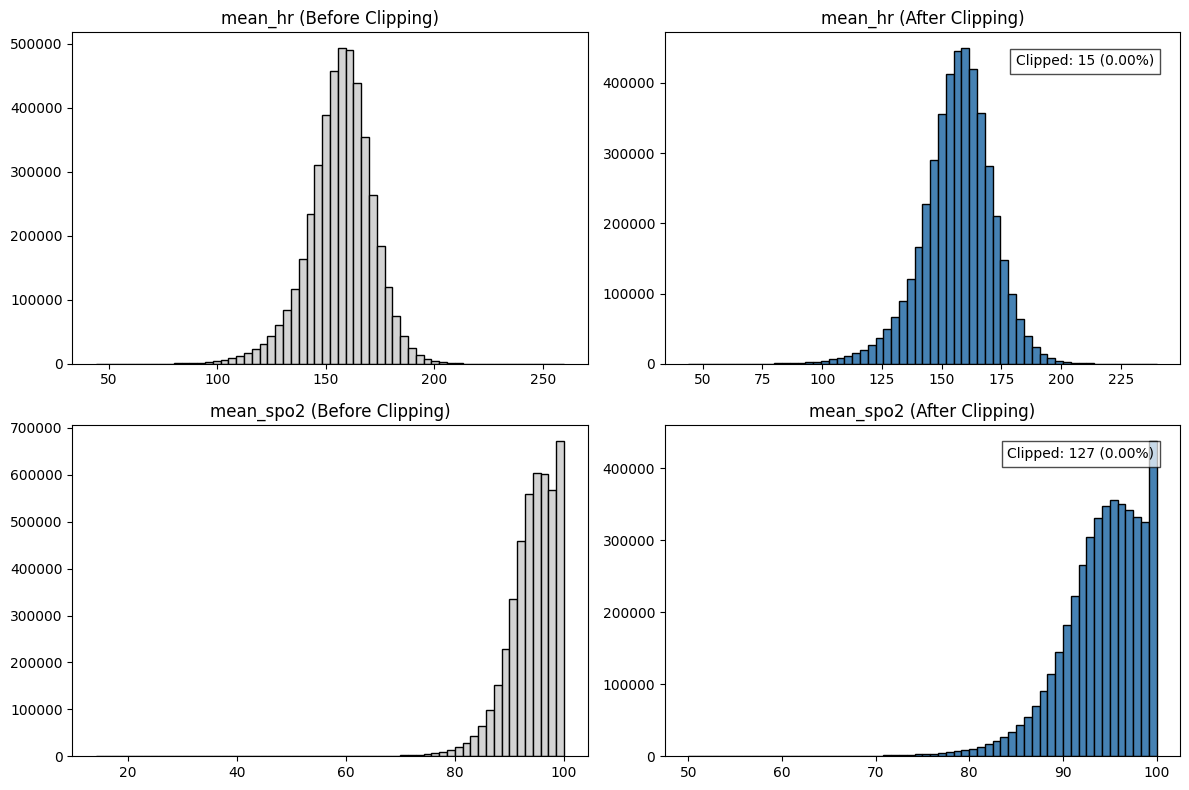
\includegraphics[width=\columnwidth]{DATA_CLIP.png}
    \caption{Before and after clipping of physiological features}
    \label{fig:data_clip}
\end{figure}


\subsubsection{Dataset Splitting and Class Imbalance Handling}\\

The dataset was divided into training, validation, and test sets at the patient level rather than at the sample level. Each infant, identified by new-id, appears in only one split, ensuring that no data from the same patient is shared across different sets. This strategy prevents data leakage caused by temporal similarity within a patient’s records and results in a more realistic evaluation scenario in which the model is tested on infants it has not encountered during training \cite{plos_ehr_sepsis,Saria2019SafeML}.

The dataset exhibits a strong class imbalance, with negative samples greatly outnumbering positive ones. Training directly on this distribution would bias the model toward predicting the negative class. To address this issue, a patient-aware undersampling strategy was employed instead of random undersampling. Each patient was treated independently to prevent infants with a large number of samples from dominating the training process \cite{Nemati2018Interpretable}.

For infected patients, negative samples were divided into near-negative samples, which are temporally close to the sepsis window and therefore more difficult to distinguish from positive cases, and far-negative samples, which are temporally distant from the event and easier to classify. A larger proportion of near-negative samples and a smaller proportion of far-negative samples were retained. For non-infected patients, only a small subset of negative samples was kept. The impact of this strategy was verified by comparing the number of patients and samples before and after undersampling, as well as by visualizing the resulting change in class distribution, as shown in Fig.~\ref{fig:patients_rows} and Fig.~\ref{fig:undersample_patientaware} \cite{los_ml_mdpi,VanWyk2019Physiomarkers}.

\begin{figure}[H]
\centering
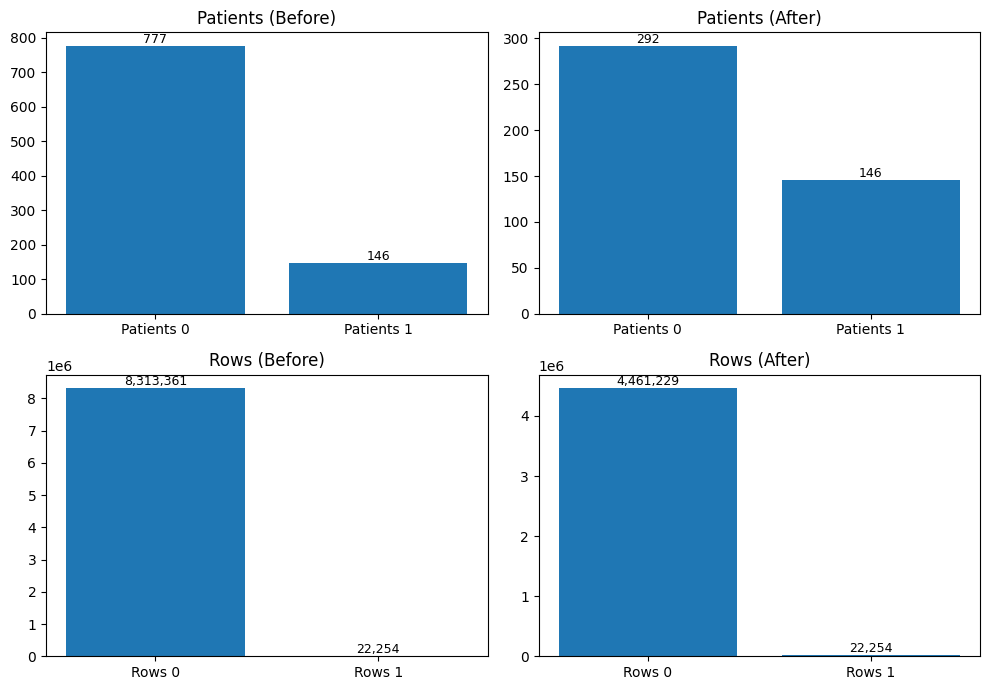
\includegraphics[width=\columnwidth]{patient_rows_before_after.png}
\caption{Patients versus rows before and after undersampling}
\label{fig:patients_rows}
\end{figure}

\begin{figure}[H]
\centering
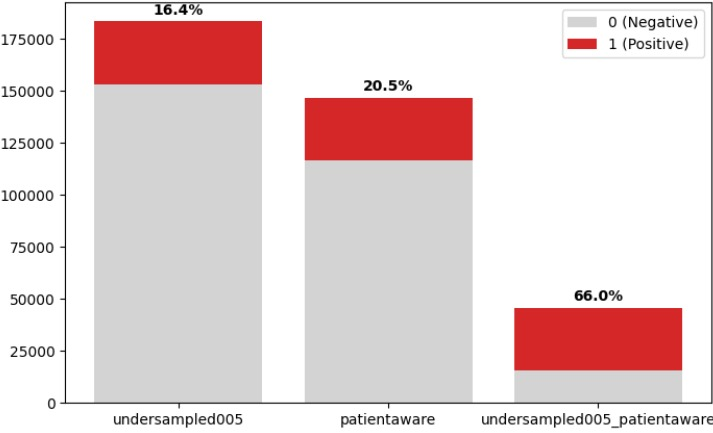
\includegraphics[width=\columnwidth]{UNDER_SAMBLE.jpeg}
\caption{Patient-aware undersampling strategy}
\label{fig:undersample_patientaware}
\end{figure}


\subsection{Temporal Sequence Creation} 

Data will be grouped by patient and sorted chronologically by timestamp (seconds\_since\_birth). Sliding windows will be generated to create fixed-length sequences:
\begin{itemize}
    \item Sequence length of 24 timesteps for LSTM-based experiments.
    \item Sequence length of 144 timesteps (approximately 24 hours at approximately 10-minute intervals) for GRU-based experiments.
\end{itemize}
During training, overlapping windows with small strides will be used to maximize data utilization. During inference and evaluation, larger strides will be applied to reduce temporal overlap and prevent inflated performance dcaused by high redundancy.


\subsection{Recurrent Neural Network Models with Attention}

Two bidirectional recurrent neural network architectures will be implemented to capture long-range temporal dependencies in physiological signals. The first model is a bidirectional Long Short-Term Memory (LSTM) network with attention, consisting of a single recurrent layer with a hidden dimension of 64 and a dropout rate of 0.3. An additive attention mechanism is applied using a linear layer to compute attention scores, followed by softmax normalization and a weighted summation of hidden states to form a context vector.\\


Both models produce a single logit output through a final fully connected layer, followed by sigmoid activation to obtain probability estimates for binary classification. Training will be performed using the BCEWithLogitsLoss function with positive class weighting to address residual class imbalance.

\begin{figure}[H]
    \centering
    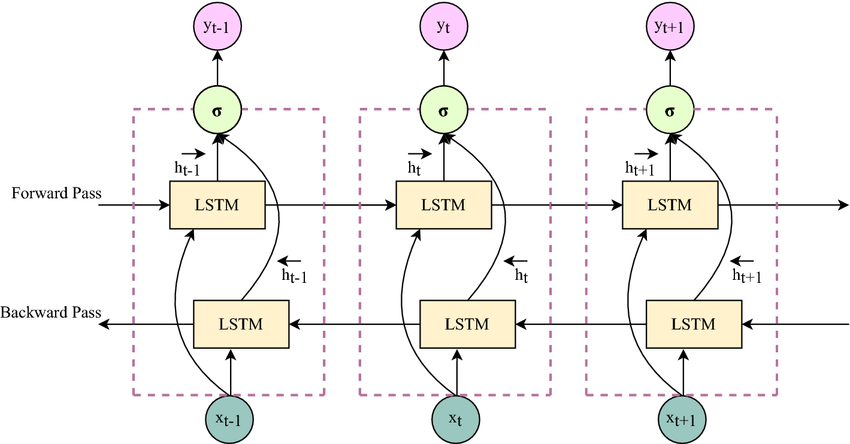
\includegraphics[width=0.5\textwidth]{Bidirectional-LSTM-architecture.png}
    \caption{Bidirectional LSTM with attention for time series. Adapted from \cite{schuster1997}.}
    \label{fig:bidirectional_lstm}
\end{figure}


\subsection{Overview of the Proposed Framework}
The proposed patient-aware framework for early neonatal sepsis prediction processes multivariate time-series physiological data (heart rate and oxygen saturation) collected from NICU monitoring systems in a clinically realistic manner.

As illustrated in Figure~\ref{fig:framework_pipeline}, the framework consists of four main stages. First, a robust patient-aware preprocessing pipeline is applied. This includes physiologically informed clipping of vital signs, median imputation (or standard scaling for deep models), patient-level splitting to prevent data leakage, and careful undersampling that preserves near-negative samples while maintaining class balance. Static demographic features such as birth weight are integrated with the extracted statistical time-series features.

Second, temporal sequence construction is performed by grouping data chronologically per patient and generating fixed-length sliding windows. For the LSTM model, sequences of length 24 timesteps are used, while the XGBoost and ensemble models operate on statistical summaries derived from longer windows (up to 144 timesteps).

Third, multiple complementary models are trained within a unified multi-model learning framework:
\begin{itemize}
    \item The XGBoost model, a powerful gradient boosting approach that leverages hand-crafted statistical features and provides high interpretability.
    \item The bidirectional LSTM model, a deep recurrent architecture that directly captures long-term temporal dependencies.
    \item A soft-voting ensemble combining Random Forest, XGBoost, and LightGBM to benefit from the complementary strengths of tree-based learners.
\end{itemize}

All models are trained under identical patient-aware conditions to ensure fair comparison.

Finally, a dedicated clinical alerting pipeline converts raw model probabilities into actionable alerts. This post-processing stage incorporates exponential moving average (EMA) smoothing ($\alpha=0.3$), $k$-of-$n$ detection ($k=2$, $n=3$), and a refractory period of 3 steps to suppress false alarms and reduce alert fatigue.

\subsection{Multi-Model Learning Framework}

\subsubsection{XGBoost Model}



The XGBoost model is employed as a powerful gradient boosting algorithm and serves as an effective model among the machine learning approaches evaluated in this study. XGBoost is an optimized implementation of gradient boosted decision trees known for its strong performance on structured tabular data, built-in regularization techniques, and efficient handling of class imbalance.

The model was trained on the 11 hand-crafted statistical and demographic features described in Section~III-A: mean heart rate (\texttt{mean\_hr}), standard deviation of heart rate (\texttt{sd\_hr}), skewness and kurtosis of heart rate, mean and standard deviation of oxygen saturation (\texttt{mean\_spo2}, \texttt{sd\_spo2}), skewness and kurtosis of SpO$_2$, maximum and minimum cross-correlation between HR and SpO$_2$ (\texttt{max\_xc\_hr\_spo2}, \texttt{min\_xc\_hr\_spo2}), and birth weight. After median imputation of any remaining missing values, the following hyperparameters were used:

\begin{itemize}
    \item \texttt{n\_estimators}: 200
    \item \texttt{max\_depth}: 4
    \item \texttt{learning\_rate}: 0.05
    \item \texttt{subsample}: 0.9
    \item \texttt{colsample\_bytree}: 0.9
    \item \texttt{objective}: binary:logistic
    \item \texttt{eval\_metric}: [\texttt{logloss}, \texttt{auc}]
    \item \texttt{scale\_pos\_weight}: 0.515 (computed as the inverse ratio of negative to positive samples in the patient-aware undersampled training set)
    \item \texttt{tree\_method}: hist with GPU acceleration (\texttt{device='cuda'})
    \item \texttt{random\_state}: 42
\end{itemize}

Training followed the same patient-aware splitting protocol used throughout the study to prevent data leakage. Model outputs were evaluated at both the individual time-window level and the patient level. To ensure clinical realism, the same post-processing pipeline was applied: exponential moving average (EMA) smoothing ($\alpha = 0.3$), $k$-of-$n$ detection ($k=2$, $n=3$), and a refractory period of 3 steps. Probability calibration was also performed using Platt scaling via \texttt{CalibratedClassifierCV} on the validation set to improve the reliability of the predicted probabilities.

This XGBoost model provided strong discriminative performance while maintaining high interpretability and computational efficiency, making it a valuable component for early neonatal sepsis prediction using multivariate statistical features.




\subsection{Proposed Ensemble Model}

\subsubsection{Overview}
In addition to evaluating individual machine learning models, this study proposes a soft-voting ensemble framework aimed at improving predictive robustness and generalization performance for early neonatal sepsis detection. The proposed ensemble integrates three complementary tree-based models, each designed to capture different aspects of the data distribution.

\subsubsection{Base Learners Configuration}
The ensemble consists of the following models:

\begin{itemize}
    \item \textbf{Random Forest (RF):} Configured with 150 estimators and a maximum depth of 7, enabling effective variance reduction while maintaining interpretability.
    
    \item \textbf{XGBoost (XGB):} Configured with 150 estimators, a maximum depth of 4, a learning rate of 0.05, and a subsample ratio of 0.9. This setup allows capturing complex non-linear relationships while mitigating overfitting.
    
    \item \textbf{LightGBM (LGBM):} Configured with 150 estimators, a maximum depth of 6, a learning rate of 0.05, and 31 leaves, leveraging a leaf-wise growth strategy for efficient learning.
\end{itemize}

\subsubsection{Ensemble Strategy and Calibration}
The base learners are combined using a soft-voting strategy implemented via a \texttt{VotingClassifier}. The predicted probabilities are aggregated using weighted averaging with weights $[1, 1.1, 1.05]$.

To ensure reliable probabilistic outputs for clinical decision-making, the ensemble is further calibrated using \texttt{CalibratedClassifierCV} with the sigmoid method (Platt Scaling) and 5-fold cross-validation. This step ensures that the predicted outputs represent well-calibrated clinical risks.

\subsubsection{Ensemble Probability Formulation}
The final ensemble probability is computed as follows:

\begin{equation}
P_{\text{ens}} = \frac{1 \cdot P_{\text{RF}} + 1.1 \cdot P_{\text{XGB}} + 1.05 \cdot P_{\text{LGBM}}}{1 + 1.1 + 1.05}
\end{equation}

\subsubsection{Feature Engineering}
The model was trained on 11 clinically relevant features extracted from 24-hour sliding windows. These include:

\begin{itemize}
    \item Heart rate statistics: mean, standard deviation, skewness, kurtosis
    \item SpO$_2$ statistics: mean, standard deviation, skewness, kurtosis
    \item Cross-correlation features: minimum and maximum correlation between heart rate and SpO$_2$
    \item Birth weight
\end{itemize}

Missing values were handled using median imputation to ensure robustness against incomplete clinical data.

\subsubsection{Post-processing Mechanism}
To enhance clinical reliability and reduce false alarm rates, a temporal k-of-n post-processing rule ($k = 5$, $n = 7$) was applied. A sepsis alert is triggered only if at least five out of the seven most recent consecutive time windows are predicted as high risk, ensuring temporal consistency and reducing the impact of transient noise.

\subsubsection{Model Evaluation Strategy}
XGBoost was evaluated both as an independent baseline model and as a component of the ensemble. This design allows for clear quantification of the ensemble gain, demonstrating how the integration of Random Forest’s variance reduction, XGBoost’s expressive modeling capacity, and LightGBM’s computational efficiency results in a more stable and robust predictive system.




\subsubsection{LSTM Model}

The Long Short-Term Memory (LSTM) network was employed 
as a unidirectional recurrent baseline model to capture 
short-term temporal dependencies within sequential 
physiological windows. Unlike bidirectional architectures, 
the unidirectional LSTM processes each input window 
strictly in the forward temporal direction, ensuring causal 
consistency with the clinical deployment scenario in which 
only past observations are available at inference time.

The model accepts a single time-step input of dimension 13, 
corresponding to the statistical features extracted from 
each 10-minute monitoring window. The architecture consists 
of two stacked LSTM layers with a hidden dimension of 128 
and a dropout rate of 0.3 applied between layers to reduce 
overfitting. The final hidden state of the last time step 
is passed through a two-layer fully connected classifier: 
a linear layer reducing dimensionality from 128 to 64, 
followed by a ReLU activation, a dropout layer 
(\(p = 0.3\)), and a final linear layer producing a single 
logit for binary classification.

The model was trained using the following configuration:

\begin{itemize}
    \item \textbf{Input dimension:} 13 features 
    (\texttt{mean\_hr}, \texttt{mean\_spo2}, 
    \texttt{sd\_hr}, \texttt{sd\_spo2}, 
    \texttt{skewness\_hr}, \texttt{skewness\_spo2}, 
    \texttt{kurtosis\_hr}, \texttt{kurtosis\_spo2}, 
    \texttt{max\_xc\_hr\_spo2}, \texttt{min\_xc\_hr\_spo2}, 
    \texttt{sub}, \texttt{sepsis\_window}, 
    \texttt{blackout\_window})

    \item \textbf{Architecture:} 2-layer unidirectional LSTM 
    (hidden size = 128, dropout = 0.3) followed by a fully 
    connected classifier (128 $\rightarrow$ 64 $\rightarrow$ 1)

    \item \textbf{Total parameters:} 213,633 (all trainable)

    \item \textbf{Loss function:} Binary Cross-Entropy with 
    Logits Loss (\texttt{BCEWithLogitsLoss}) with a positive 
    class weight of 0.5149, computed as the inverse ratio of 
    negative to positive samples in the patient-aware 
    undersampled training set

    \item \textbf{Optimizer:} AdamW with learning rate 
    $= 1 \times 10^{-3}$ and weight decay 
    $= 1 \times 10^{-4}$

    \item \textbf{Scheduler:} ReduceLROnPlateau with a 
    reduction factor of 0.5 and patience of 5 epochs, 
    monitoring validation PR-AUC

    \item \textbf{Early stopping:} Patience of 10 epochs 
    based on validation PR-AUC

    \item \textbf{Batch size:} 256

    \item \textbf{Maximum epochs:} 50

    \item \textbf{Training device:} CUDA-enabled GPU 
    (NVIDIA GeForce RTX 3050 Ti Laptop GPU)

    \item \textbf{Random seed:} 42
\end{itemize}

Probability calibration was performed post-training using 
Platt scaling applied to the validation set, improving the 
reliability of predicted probabilities for downstream 
clinical use. The classification threshold was subsequently 
optimized on the calibrated validation probabilities using 
the F2-score ($\beta = 2$) to prioritize recall in this 
clinically imbalanced setting. The optimal threshold was 
determined to be 0.169, yielding a validation F2-score 
of 0.5733.

Training followed the same patient-aware splitting protocol 
used throughout the study to prevent data leakage. Model 
outputs were evaluated at both the individual time-window 
level and the patient level, providing a comprehensive 
assessment of predictive performance under clinically 
realistic conditions.

This LSTM model provided strong discriminative performance 
while capturing temporal dependencies in physiological 
signals, making it a valuable recurrent baseline for early 
neonatal sepsis prediction.


\section{Experimental Design}

\subsection{Baseline Model Comparison}
All models were trained and evaluated under identical conditions using the same patient-aware data splits, the same statistical features, the same preprocessing pipeline, and the same post-processing and calibration procedures. This consistent experimental design ensures a fair comparison and highlights the relative strengths of different learning paradigms for the early neonatal sepsis forecasting task.

The XGBoost model, as a classical gradient boosting approach, demonstrated strong performance with high computational efficiency and excellent interpretability. It achieved competitive window-level metrics and solid patient-level sensitivity, particularly excelling in scenarios where feature importance and transparency are critical.

The bidirectional LSTM model showed superior capability in capturing long-term temporal dependencies within the physiological time-series. This resulted in improved PR-AUC and strong patient-level detection rates, confirming the advantage of recurrent architectures for modeling the gradual progression of sepsis.

The soft-voting ensemble (Random Forest + XGBoost + LightGBM) provided the best overall balance between sensitivity and specificity. By combining the complementary strengths of its base learners, the ensemble achieved higher robustness and more stable alerts compared to the individual models.

Across all models, the application of the clinical alerting pipeline (EMA smoothing, $k$-of-$n$ detection, and refractory period) significantly enhanced practical usability by reducing false alarms while preserving clinically meaningful lead times. These results demonstrate that no single paradigm dominates; rather, each offers distinct advantages that can be leveraged depending on deployment priorities (interpretability, temporal modeling, or overall robustness).

\subsection{Feature Ablation Methodology}
 A systematic feature ablation study was conducted to evaluate the contribution of each individual feature to model performance. For each model, one feature was sequentially removed while all other experimental conditions—including preprocessing, patient-aware splitting, hyperparameters, and post-processing—were held constant. The model was retrained and evaluated on the validation set using the F$_2$-score as the primary metric to emphasize recall in this imbalanced early-warning task.

The ablation results revealed clear differences in feature sensitivity across the three modeling paradigms:

\begin{itemize}
    \item For the \textbf{XGBoost model}, heart-rate variability features exerted the strongest influence. Removal of \texttt{sd\_hr} (standard deviation of heart rate) and \texttt{skewness\_hr} produced the largest degradation in F$_2$-score, confirming the clinical importance of increased variability as an early indicator of sepsis. Cross-correlation features (\texttt{max\_xc\_hr\_spo2} and \texttt{min\_xc\_hr\_spo2}) and birth weight also showed substantial contribution, while kurtosis features had comparatively smaller impact.

    \item The \textbf{bidirectional LSTM model} demonstrated higher sensitivity to temporal statistical features, particularly \texttt{mean\_spo2} and \texttt{sd\_hr}. This aligns with the model’s ability to capture long-term dependencies, making it more affected by the removal of features that reflect gradual physiological changes.

    \item The \textbf{soft-voting ensemble} proved to be the most robust to feature removal. Although \texttt{sd\_hr}, \texttt{skewness\_hr}, and \texttt{mean\_spo2} remained the most influential, performance degradation was generally more gradual compared to the standalone models. This robustness stems from the complementary strengths of Random Forest, XGBoost, and LightGBM, allowing the ensemble to partially compensate when individual features are unavailable.
\end{itemize}

These findings are consistent with the SHAP and permutation importance analyses performed on each model. Overall, heart-rate variability and oxygen saturation statistics consistently emerged as the most critical features across all three approaches, validating the clinical relevance of the engineered time-series features used in this study.

\subsection{Model-Specific Evaluation}

The feature ablation process was applied consistently across all models to evaluate how each model responds to feature removal and to analyze model-specific feature sensitivity. For every experiment, one feature was sequentially removed while all other experimental conditions—including preprocessing pipeline, patient-aware data splitting, hyperparameters, loss function, and post-processing steps—were held fixed. The model was then retrained from scratch and evaluated on the validation set using the F2-score as the primary performance metric to prioritize recall in this highly imbalanced early sepsis prediction task.


\FloatBarrier

\paragraph{XGBoost Model}


Feature ablation applied to the XGBoost model revealed that heart-rate variability features exert the strongest influence on predictive performance. Specifically, removal of \texttt{sd\_hr} and \texttt{skewness\_hr} produced the largest degradation in F$_2$-score, confirming their critical role in early sepsis detection.

The cross-correlation features (\texttt{max\_xc\_hr\_spo2} and \texttt{min\_xc\_hr\_spo2}) also demonstrated meaningful contributions, while \texttt{birth\_weight} showed a moderate but consistent impact. In contrast, kurtosis-based and SpO$_2$ variability features exhibited comparatively smaller influence.

These findings are illustrated in Figure~\ref{fig:XGBoost_FAblaltion}, which shows the validation F$_2$-score after removing each feature, and are summarized numerically in Table~\ref{tab:XGBoost_FAblaltion}.

\begin{figure}[H]
    \centering
    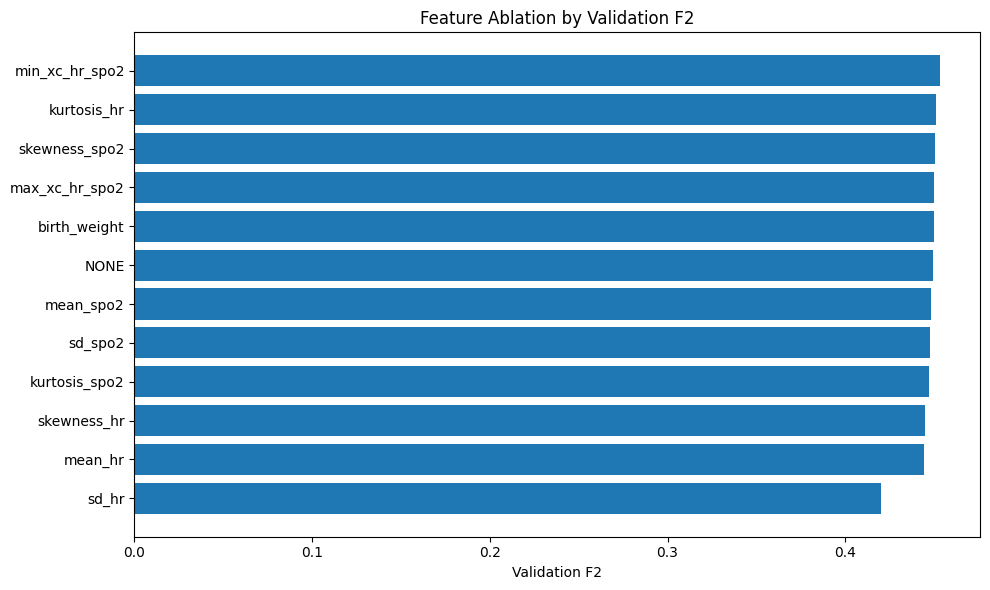
\includegraphics[width=0.85\linewidth]{XGBoost_FAblaltion.png}
    \caption{Feature ablation analysis for the XGBoost model showing validation F$_2$-score after removing each feature. Lower scores indicate higher feature importance.}
    \label{fig:xgb_ablation}
\end{figure}

\begin{table}[H]
\centering
\caption{Feature ablation results for the XGBoost model (validation set).}
\label{tab:xgb_ablation}
\renewcommand{\arraystretch}{1.1}

\resizebox{\linewidth}{!}{
\begin{tabular}{|l|c|c|c|c|c|}
\hline
\textbf{Removed Feature} & \textbf{Accuracy} & \textbf{Precision} & \textbf{Recall} & \textbf{F1} & \textbf{F2} \\
\hline
min\_xc\_hr\_spo2 & 0.5365 & 0.1684 & 0.7850 & 0.2773 & 0.4532 \\
\hline
kurtosis\_hr & 0.5511 & 0.1705 & 0.7667 & 0.2790 & 0.4512 \\
\hline
skewness\_spo2 & 0.5452 & 0.1692 & 0.7710 & 0.2775 & 0.4505 \\
\hline
max\_xc\_hr\_spo2 & 0.5304 & 0.1664 & 0.7847 & 0.2746 & 0.4502 \\
\hline
birth\_weight & 0.4757 & 0.1579 & 0.8372 & 0.2657 & 0.4500 \\
\hline
NONE (All features) & 0.5568 & 0.1711 & 0.7579 & 0.2792 & 0.4496 \\
\hline
mean\_spo2 & 0.5100 & 0.1625 & 0.8008 & 0.2702 & 0.4485 \\
\hline
sd\_spo2 & 0.5027 & 0.1612 & 0.8063 & 0.2687 & 0.4478 \\
\hline
kurtosis\_spo2 & 0.5402 & 0.1673 & 0.7693 & 0.2749 & 0.4474 \\
\hline
skewness\_hr & 0.4914 & 0.1586 & 0.8106 & 0.2653 & 0.4448 \\
\hline
mean\_hr & 0.5112 & 0.1616 & 0.7911 & 0.2683 & 0.4446 \\
\hline
sd\_hr & 0.3718 & 0.1376 & 0.8626 & 0.2373 & 0.4199 \\
\hline
\end{tabular}
}

\end{table}\\

\paragraph{Proposed Ensemble Model}

The proposed soft-voting ensemble (RF + XGBoost + LightGBM), trained on the 11-dimensional feature set derived from 24-hour sliding windows, demonstrated greater overall robustness to feature removal compared to the standalone XGBoost model. When individual features were sequentially ablated, the performance degradation was consistently more gradual in the ensemble than in any single base learner.

This robustness stems directly from the complementary strengths of the three learners: Random Forest provides variance reduction through bagging, XGBoost offers powerful sequential error correction, and LightGBM utilizes an efficient leaf-wise growth strategy.

Even when influential features such as \textit{sd\_hr}, \textit{mean\_hr}, and SpO\textsubscript{2} variability statistics (e.g., \textit{sd\_spo2}, \textit{skewness\_spo2}) were removed, the ensemble was able to partially compensate using the remaining features.

The combination of statistical measures (mean, standard deviation, skewness, and kurtosis), along with cross-correlation features between heart rate and SpO\textsubscript{2}, consistently emerged as important for early sepsis detection. In addition, \textit{birth\_weight} provided modest but useful contextual information.

These findings were supported by the feature ablation study, which showed that the ensemble maintains higher F2-score stability under feature removal, confirming its superior generalization ability and clinical reliability in scenarios where certain physiological data may be missing or noisy.

.

\FloatBarrier
% ====================== SHAP Summary Plot + Feature Ablation Table ======================
\begin{figure}[H]
    \centering
    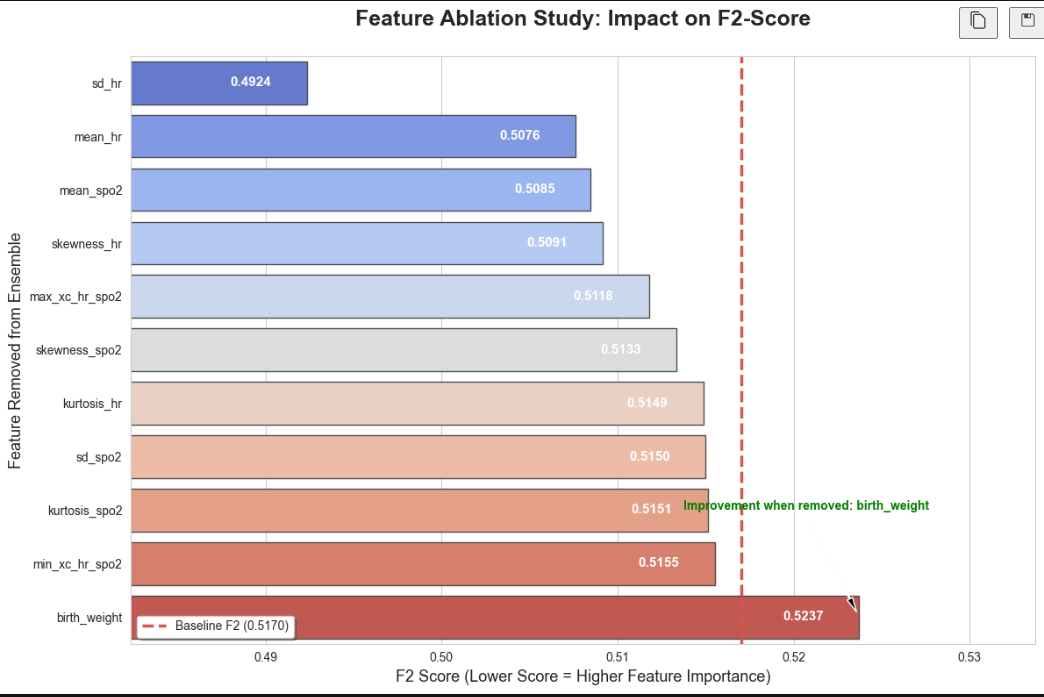
\includegraphics[width=0.92\linewidth]{ensemble_feature_importance}
    \caption{ plot showing the feature importance ranking obtained from the proposed ensemble model.}
    \label{fig:shap_ensemble}
\end{figure}

% Feature Ablation Table - Placed directly below the SHAP plot
\begin{table}[H]
    \centering
    \caption{Full Feature Ablation Results for the Proposed Ensemble Model (Sorted by F2 Impact)}
    \label{tab:full_feature_ablation}
    \renewcommand{\arraystretch}{1.2}
    \resizebox{\linewidth}{!}{
    \begin{tabular}{|l|c|c|c|c|c|}
        \hline
        \textbf{Removed Feature} & \textbf{ROC AUC} & \textbf{PR AUC} & \textbf{F2-Score} & \textbf{Patient Sens.} & \textbf{F2 Drop} \\ 
        \hline
        sd\_hr            & 0.6631 & 0.2414 & 0.4924 & 100\% & 0.0247 \\ \hline
        mean\_hr          & 0.6924 & 0.2589 & 0.5076 & 100\% & 0.0094 \\ \hline
        mean\_spo2        & 0.6985 & 0.2668 & 0.5085 & 100\% & 0.0085 \\ \hline
        skewness\_hr      & 0.6999 & 0.2666 & 0.5091 & 100\% & 0.0079 \\ \hline
        max\_xc\_hr\_spo2  & 0.6981 & 0.2505 & 0.5118 & 100\% & 0.0052 \\ \hline
        skewness\_spo2    & 0.7051 & 0.2679 & 0.5133 & 100\% & 0.0037 \\ \hline
        kurtosis\_hr      & 0.7042 & 0.2657 & 0.5149 & 100\% & 0.0021 \\ \hline
        sd\_spo2          & 0.7044 & 0.2657 & 0.5150 & 100\% & 0.0020 \\ \hline
        kurtosis\_spo2    & 0.7034 & 0.2669 & 0.5151 & 100\% & 0.0019 \\ \hline
        min\_xc\_hr\_spo2  & 0.7037 & 0.2651 & 0.5155 & 100\% & 0.0015 \\ \hline
        birth\_weight     & 0.7162 & 0.2790 & 0.5237 & 100\% & -0.0067 \\ \hline
        \hline
        \textbf{NONE (Baseline)} & \textbf{0.7056} & \textbf{0.2644} & \textbf{0.5170} & \textbf{4.55\%} & \textbf{0.0000} \\ \hline
    \end{tabular}
    }
\end{table}

\paragraph{LSTM Model}

A systematic feature ablation study was conducted on the LSTM model 
following the same protocol applied to all other models in this framework. 
Starting from a baseline configuration trained on all 13 input features, 
one feature was removed at a time and the model was retrained from scratch 
under identical conditions—same patient-aware splits, same preprocessing 
pipeline, same architecture, same hyperparameters, and same post-processing 
steps. Performance was evaluated on the held-out test set using the 
$F_2$-score as the primary metric, alongside AU-ROC and PR-AUC.

Table~\ref{tab:lstm_ablation} summarizes the results of the ablation 
experiments, reporting the change in AU-ROC ($\Delta$ROC), PR-AUC 
($\Delta$PR), and $F_2$-score ($\Delta F_2$) relative to the baseline 
for each removed feature.

\begin{table}[H]
\centering
\caption{LSTM feature ablation results. Each row reports performance 
when the indicated feature is removed. $\Delta$ values represent the 
difference from the 13-feature baseline 
(ROC = 0.8683, PR = 0.5413, F$_2$ = 0.5550).}
\label{tab:lstm_ablation}
\renewcommand{\arraystretch}{1.2}
\resizebox{\linewidth}{!}{
\begin{tabular}{|l|c|c|c|c|c|c|}
\hline
\textbf{Removed Feature} & \textbf{ROC-AUC} & \textbf{$\Delta$ROC} & \textbf{PR-AUC} & \textbf{$\Delta$PR} & \textbf{F$_2$} & \textbf{$\Delta$F$_2$} \\
\hline
None (Baseline) & 0.8683 & -- & 0.5413 & -- & 0.5550 & -- \\
\hline
\texttt{mean\_hr}        & 0.8652 & $-$0.0031 & 0.5428 & $+$0.0015 & 0.5558 & $+$0.0008 \\
\hline
\texttt{mean\_spo2}      & 0.8644 & $-$0.0039 & 0.5391 & $-$0.0022 & 0.5554 & $+$0.0004 \\
\hline
\texttt{sd\_hr}          & 0.8478 & $-$0.0205 & 0.5360 & $-$0.0053 & 0.5558 & $+$0.0008 \\
\hline
\texttt{sd\_spo2}        & 0.8692 & $+$0.0009 & 0.5427 & $+$0.0014 & 0.5544 & $-$0.0006 \\
\hline
\texttt{skewness\_hr}    & 0.8672 & $-$0.0011 & 0.5428 & $+$0.0015 & 0.5557 & $+$0.0007 \\
\hline
\texttt{skewness\_spo2}  & 0.8691 & $+$0.0008 & 0.5403 & $-$0.0010 & 0.5557 & $+$0.0007 \\
\hline
\texttt{kurtosis\_hr}    & 0.8692 & $+$0.0009 & 0.5425 & $+$0.0012 & 0.5557 & $+$0.0007 \\
\hline
\texttt{kurtosis\_spo2}  & 0.8685 & $+$0.0002 & 0.5409 & $-$0.0004 & 0.5559 & $+$0.0009 \\
\hline
\texttt{max\_xc\_hr\_spo2} & 0.8655 & $-$0.0028 & 0.5372 & $-$0.0041 & 0.5557 & $+$0.0007 \\
\hline
\texttt{min\_xc\_hr\_spo2} & 0.8681 & $-$0.0002 & 0.5404 & $-$0.0009 & 0.5557 & $+$0.0007 \\
\hline
\texttt{sub}             & 0.8688 & $+$0.0005 & 0.5403 & $-$0.0010 & 0.5553 & $+$0.0003 \\
\hline
\texttt{sepsis\_window}  & 0.7370 & $-$0.1313 & 0.0325 & $-$0.5088 & 0.1149 & $-$0.4401 \\
\hline
\texttt{blackout\_window}& 0.8608 & $-$0.0075 & 0.5373 & $-$0.0040 & 0.5558 & $+$0.0008 \\
\hline
\end{tabular}
}
\end{table}

The ablation results reveal a clear hierarchy of feature importance 
for the LSTM model. The \texttt{sepsis\_window} feature exhibited by 
far the largest impact upon removal, producing a dramatic drop in 
AU-ROC of 0.1313 and a collapse in PR-AUC of 0.5088, reducing it 
from 0.5413 to merely 0.0325. This confirms that \texttt{sepsis\_window} 
encodes critical temporal context that the LSTM relies upon heavily 
for discriminating between sepsis-risk and non-risk windows.

Among the physiological signal features, \texttt{sd\_hr} (standard 
deviation of heart rate) demonstrated the most meaningful contribution, 
with its removal causing a drop in AU-ROC of 0.0205 and a reduction 
in PR-AUC of 0.0053. This is consistent with the well-established 
clinical finding that increased heart rate variability is an early 
physiological marker of sepsis in neonates 
\cite{hero_monitoring,vital_sign_ml}. The \texttt{blackout\_window} 
feature also showed a moderate contribution ($\Delta$ROC $= -0.0075$, 
$\Delta$PR $= -0.0040$), while \texttt{mean\_spo2} and 
\texttt{max\_xc\_hr\_spo2} exhibited smaller but consistent 
negative impacts upon removal.

In contrast, features including \texttt{sd\_spo2}, 
\texttt{skewness\_spo2}, \texttt{kurtosis\_hr}, and \texttt{sub} 
showed negligible or marginally positive effects when removed, 
suggesting that the LSTM learns redundant representations for 
these signals and can compensate for their absence through 
the remaining feature set.

These findings are consistent with the broader literature on 
neonatal sepsis prediction, where heart rate variability and 
cardiorespiratory coupling have been consistently identified 
as the most clinically informative physiological markers 
\cite{hero_monitoring,Shashikumar2017EarlySepsis}.


\subsubsection{Comparative Feature Sensitivity}

A comparative analysis of feature sensitivity across all models reveals both consistent patterns and model-specific behaviors in how physiological features contribute to early sepsis prediction.

Across all models, heart rate variability features—particularly \texttt{sd\_hr}—consistently emerged as the most influential predictors. The removal of this feature resulted in noticeable performance degradation in XGBoost, the deep learning model, and the LSTM, confirming its strong clinical relevance as an early indicator of sepsis.

Similarly, cross-correlation features between heart rate and oxygen saturation (\texttt{max\_xc\_hr\_spo2} and \texttt{min\_xc\_hr\_spo2}) demonstrated moderate importance across multiple models, highlighting the significance of cardiorespiratory coupling patterns.

However, differences between models were also observed. The LSTM model showed a strong dependence on temporal context features such as \texttt{sepsis\_window}, which caused a substantial drop in performance when removed. In contrast, the deep learning MLP model relied more heavily on distributional statistics (e.g., skewness and mean), reflecting its ability to capture nonlinear relationships in static feature representations.

The ensemble model exhibited the highest robustness to feature removal, with more gradual performance degradation across all ablation experiments. This indicates that combining multiple learners allows the model to compensate for missing information by leveraging complementary feature representations.

Overall, this comparative analysis demonstrates that while certain features are universally important, each model exhibits distinct sensitivity patterns. These findings highlight the advantage of multi-model frameworks in achieving both high predictive performance and resilience to missing or noisy clinical data.



\section{Experimental Setup}
Python 3 will be used to implement and evaluate the proposed framework. The PyTorch deep learning library will support both model development and training. Pandas and NumPy will handle data processing and preprocessing, while Scikit-learn will be utilized for performance metric computation, MinMaxScaler feature scaling, and Platt scaling probability calibration. Matplotlib will visualize reliability diagrams, confusion matrices, and training curves. To facilitate efficient training of recurrent neural network models, CUDA-enabled GPU hardware will accelerate all experiments.\\

The Adam optimizer will train the models with an initial learning rate of 0.001. StepLR will be adopted for the LSTM model, and cosine annealing will be applied for the GRU model to implement learning rate scheduling. To enhance training stability in the GRU experiments, mixed-precision training (AMP) and gradient clipping with a maximum norm of 5.0 will be employed. To mitigate overfitting, early stopping will be applied with a patience of three epochs for the LSTM model based on validation loss and four to ten epochs for the GRU model based on validation F2-score.

\subsection{Dataset Description}

\subsubsection{Data Source and Population}
The dataset utilized in this research was gathered from the Neonatal Intensive Care Unit (NICU) at the University of Virginia from 2012 to 2021 \cite{Moorman2023CardiorespiratorySepsis}. The dataset comprises physiological monitoring information from premature newborns admitted to the NICU, specifically concentrating on those with very low birth weight as outlined in the original cohort. The dataset comprises continuously recorded heart rate (HR) and oxygen saturation (SpO$_2$) signals obtained from typical bedside monitors during routine clinical care.

\subsubsection{Signal Processing and Feature Representation}
Following the data acquisition and preprocessing technique outlined in previous research \cite{Moorman2023CardiorespiratorySepsis}, continuous HR and SpO$_2$ signals were uniformly resampled to 0.5 Hz to maintain consistent temporal resolution across all recordings. The signals were divided into non-overlapping intervals of 10 minutes, a duration selected to encapsulate short-term physiological variability while ensuring resilience to transient artifacts \cite{hero_monitoring}.

Every 10-minute interval was encapsulated as a singular tabular entry utilizing statistical descriptors independently extracted from the HR and SpO$_2$ signals. This terminology encompasses measures of central tendency (mean), dispersion (standard deviation), and higher-order moments (skewness and kurtosis), which together define the distributional characteristics of the signals within each window. Furthermore, the maximum and minimum cross-correlation coefficients between HR and SpO$_2$ were calculated to elucidate cardiorespiratory coupling patterns that have demonstrated utility in early sepsis identification \cite{hero_monitoring,los_ml_mdpi}.

Static demographic characteristics, such as biological sex and birth weight, were included at the individual patient level. The attributes were integrated with the time-series features utilizing a unique patient identity and duplicated over all relevant windows to furnish contextual patient information in conjunction with the dynamic physiological features. Following demographic filtering, data for 438 patients was obtained and incorporated into the final feature table.

\subsubsection{Data Quality Assessment}
In the preliminary data characterization phase, fundamental quality assessments were conducted on the raw characteristics before model training. A limited quantity of windows displayed physiologically implausible readings, with 15 windows indicating out-of-range mean heart rate values and 127 windows presenting invalid mean SpO$_2$ values. Despite constituting a minimal portion of the entire dataset, these cases prompted the use of physiologically informed value clipping during preprocessing to guarantee numerical stability and clinical plausibility \cite{Saria2019SafeML}.

\subsubsection{Label Definition}
Each time interval is linked to a binary designation denoting sepsis state. The original label, \textit{sepsis\_window}, indicates whether a window aligns with a clinically established late-onset sepsis (LOS) interval, determined by culture-positive blood samples and antibiotic treatment criteria \cite{Moorman2023CardiorespiratorySepsis,cnn_psd_sepsis}.

To enable early warning prediction, an additional forecasting label, \textit{y\_forecast\_24h}, was constructed. This label assigns a positive class to windows occurring within a 24-hour horizon preceding a confirmed sepsis event, formally defined as
\begin{equation}
y_{\text{forecast\_24h}}(t) =
\begin{cases}
1, & \text{if } 0 < t_{\text{sepsis}} - t \leq 24~\text{hours}, \\
0, & \text{otherwise}.
\end{cases}
\end{equation}

\subsubsection{Dataset Statistics}
Employing the original \textit{sepsis\_window} formulation, the dataset comprised 15,352 positive time windows. Upon the use of the forecasting label \textit{y\_forecast\_24h}, the quantity of positive windows rose to 30,178. This augmentation signifies the deliberate broadening of the positive class to encompass physiologically pertinent pre-sepsis intervals, hence allowing the model to discern early warning indicators rather than identifying sepsis only post-clinical onset \cite{Moorman2023CardiorespiratorySepsis}.

Figure~\ref{fig:gender_distribution} illustrates the patient-level distribution of biological sex across sepsis and non-sepsis groups, indicating no substantial imbalance between the two cohorts.

\begin{figure}[t]
\centering
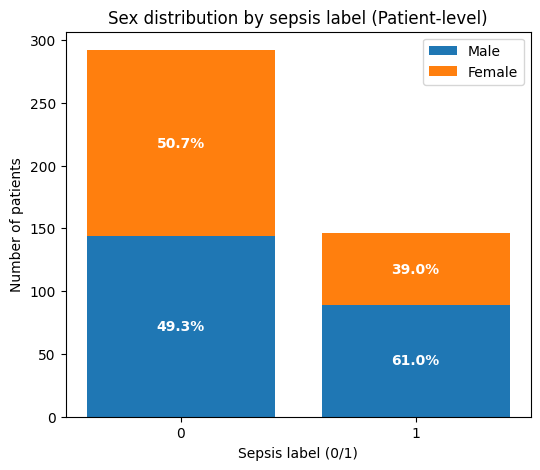
\includegraphics[width=0.9\linewidth]{gender_distribution_patient_level.png}
\caption{Patient-level distribution of biological sex across sepsis and non-sepsis groups.}
\label{fig:gender_distribution}
\end{figure}

\subsubsection{Patient-Aware Splitting}
A patient-aware splitting approach was utilized to avert information leakage between experimental splits. All windows related to a certain patient were exclusively allocated to either the training, validation, or test set. This technique embodies a pragmatic clinical implementation scenario, wherein early warning models are utilized on novel patients instead of subsequent assessments of the same individual \cite{Che2018RNNMissing}.


\subsection{Post-Processing for Practical Early Warning System}

The raw model probabilities were converted into a clinically deployable alerting mechanism using a multi-stage post-processing pipeline. To reduce short-term noise in prediction probabilities, an exponential moving average (EMA) with a smoothing factor of $\alpha \approx 0.20$ was applied. A $k$-of-$n$ detection rule was then used, triggering an alert when $k$ high-probability predictions (e.g., $k=2$) occurred within $n$ consecutive time steps (e.g., $n=3$). Following the initial alert, a refractory period was imposed to suppress subsequent alerts for a fixed duration (e.g., 12 steps).

This design enhances the clinical usability of the proposed early warning system by reducing false positives and alert fatigue.



\subsection{Evaluation Protocol}

The model’s predictions at the patient level will be interpreted in terms of correct and incorrect clinical outcomes. A correct positive (TP) indicates an infant who developed sepsis and for whom the model triggered at least one alert prior to the onset of infection. A false positive (FP) represents an uninfected infant for whom an alert was incorrectly triggered. A true negative (TN) represents an uninfected infant for whom no alert was triggered, while a false negative (FN) indicates an infected infant for whom the model failed to generate any alert before the onset of sepsis.

The model’s performance will be evaluated at both the time window and patient levels, with the primary focus on the patient level (defined as any positive alert per patient) to better reflect real-world clinical benefit.

At the window level, evaluation metrics will include accuracy, precision, recall, F1-score, area under the receiver operating characteristic curve (AU-ROC), and area under the precision–recall curve (AUPRC). Accuracy is defined as
\begin{equation}
\text{Accuracy} = \frac{\text{TP} + \text{TN}}{\text{TP} + \text{TN} + \text{FP} + \text{FN}},
\end{equation}
precision is defined as
\begin{equation}
\text{Precision} = \frac{\text{TP}}{\text{TP} + \text{FP}},
\end{equation}
recall is defined as
\begin{equation}
\text{Recall} = \frac{\text{TP}}{\text{TP} + \text{FN}},
\end{equation}
and the F1-score is defined as
\begin{equation}
\text{F1-score} = 2 \times \frac{\text{Precision} \times \text{Recall}}{\text{Precision} + \text{Recall}}.
\end{equation}

Patient-level evaluation, which represents the primary focus of this study, will comprise sensitivity, specificity, positive predictive value (PPV), negative predictive value (NPV), and lead time. Sensitivity is computed as
\begin{equation}
\text{Sensitivity} = \frac{\text{TP}}{\text{TP} + \text{FN}},
\end{equation}
specificity is defined as as\begin{equation}
\text{Specificity} = \frac{\text{TN}}{\text{TN} + \text{FP}},
\end{equation}
PPV is defined as\begin{equation}
\text{PPV} = \frac{\text{TP}}{\text{TP} + \text{FP}},
\end{equation}
and NPV is defined as\begin{equation}
\text{NPV} = \frac{\text{TN}}{\text{TN} + \text{FN}}.
\end{equation}

Lead time will be calculated as the time difference (in hours) between the first model alert and the true sepsis onset:
\begin{equation}
\text{Lead time} = \frac{t_{\text{event}} - t_{\text{alert}}}{3600}.
\end{equation}

Threshold optimization will be performed on the validation set by prioritizing the F$_2$-score ($\beta = 2$) to emphasize recall over precision, defined as
\begin{equation}
F_\beta = (1 + \beta^2)\frac{\text{Precision} \times \text{Recall}}{\beta^2 \times \text{Precision} + \text{Recall}}.
\end{equation}

Additional evaluation will include probabilistic calibration using the Brier score, defined as
\begin{equation}
\text{Brier score} = \frac{1}{N} \sum_{i=1}^{N} (p_i - o_i)^2,
\end{equation}
where $p_i$ denotes the predicted probability and $o_i \in \{0,1\}$ represents the true outcome.
Reliability diagrams will be used to visualize calibration performance, and optional Platt scaling will be applied using logistic regression on validation probabilities to further improve probability calibration.

\section{Results}

\subsection{XGBoost Model}

The performance of the XGBoost model is summarized in Table~\ref{tab:xgboost_performance}. Figures~\ref{fig:xgb_confusion}, \ref{fig:xgb_roc}, \ref{fig:xgb_pr}, and \ref{fig:xgb_calibration} further illustrate the classification behavior, discriminative ability, precision--recall trade-off, and probability calibration of the model.

\begin{table}[htbp]
\centering
\caption{Performance of the XGBoost model across different settings (window-level and patient-level metrics).}
\label{tab:xgboost_performance}

\renewcommand{\arraystretch}{1.2}

\textbf{Window-level Metrics}\\[0.5em]

\resizebox{\linewidth}{!}{
\begin{tabular}{|l|c|c|c|c|c|c|c|c|c|}
\hline
\textbf{Setting} & \textbf{Threshold} & \textbf{Accuracy} & \textbf{Precision} & \textbf{Recall} & \textbf{F1-score} & \textbf{F2-score} & \textbf{AU-ROC} & \textbf{AUPRC} & \textbf{Brier Score} \\
\hline
Raw & 0.40 & 0.556 & 0.208 & 0.738 & 0.325 & 0.489 & 0.689 & 0.262 & 0.214 \\
\hline
Post-processed & 0.40 & 0.774 & 0.203 & 0.191 & 0.197 & 0.193 & 0.711 & 0.306 & 0.203 \\
\hline
Calibrated & 0.09 & 0.531 & 0.202 & 0.759 & 0.319 & 0.489 & 0.689 & 0.262 & 0.118 \\
\hline
Calibrated + Post-processed & 0.09 & 0.758 & 0.185 & 0.196 & 0.190 & 0.194 & 0.707 & 0.302 & 0.117 \\
\hline
\end{tabular}
}

\vspace{1em}

\textbf{Patient-level Metrics}\\[0.5em]

\resizebox{\linewidth}{!}{
\begin{tabular}{|l|c|c|c|c|}
\hline
\textbf{Setting} & \textbf{Patient Sensitivity} & \textbf{Patient Specificity} & \textbf{Detection Rate} & \textbf{Median Lead Time (hours)} \\
\hline
Raw & 95.45\% & 27.27\% & 95.45\% & 257.3 \\
\hline
Post-processed & 86.36\% & 45.45\% & 86.36\% & 255.5 \\
\hline
Calibrated & 95.45\% & 25.00\% & 95.45\% & 258.2 \\
\hline
Calibrated + Post-processed & 90.91\% & 40.91\% & 86.36\% & 257.3 \\
\hline
\end{tabular}
}
\end{table}





\begin{table}[H]
\centering
\caption{Clinical alerting pipeline parameters and achieved performance for the XGBoost model.}
\label{tab:xgboost_alert_pipeline}

\renewcommand{\arraystretch}{1.3}

\resizebox{\linewidth}{!}{
\begin{tabular}{|l|l|l|}
\hline
\textbf{Component} & \textbf{Parameter} & \textbf{Value} \\
\hline

Exponential Moving Average (EMA) 
& Smoothing factor ($\alpha$) 
& 0.3 \\
\hline

$k$-of-$n$ detection rule 
& $k$ / $n$ 
& 2 / 3 \\
\hline

Refractory period 
& Steps after each alert 
& 3 \\
\hline

Threshold optimization 
& Primary metric 
& F$_2$-score ($\beta=2$) \\
\hline

Probability calibration 
& Method 
& Platt scaling (CalibratedClassifierCV) \\
\hline

\multicolumn{3}{|l|}{\textbf{Achieved Results (Test Set)}} \\
\hline

Median lead time (Raw) & - & 257.3 hours \\
\hline
Median lead time (Post-processed) & - & 255.5 hours \\
\hline
Median lead time (Calibrated + Post-processed) & - & 257.3 hours \\
\hline
Patient-level sensitivity (best) & - & 95.45\% \\
\hline
False alarm reduction (post-processing) & - & Significant improvement in alert stability \\
\hline

\end{tabular}
}

\end{table}
The results presented in Table~\ref{tab:xgboost_alert_pipeline} summarize both the configuration of the clinical alerting pipeline and its impact on early sepsis detection performance.

The exponential moving average (EMA) with a smoothing factor of $\alpha = 0.3$ was applied to reduce short-term fluctuations in predicted probabilities, resulting in more stable temporal predictions. The $k$-of-$n$ detection rule ($2$ out of $3$) was used to ensure that alerts are triggered only when consistent high-risk predictions are observed, thereby reducing spurious alarms.

Additionally, a refractory period of three time steps was introduced to prevent repeated alerts within a short time window, effectively mitigating alarm fatigue in clinical settings. Threshold optimization was performed using the F$_2$-score ($\beta = 2$), prioritizing recall to ensure early detection of sepsis cases.

Probability calibration using Platt scaling further improved the reliability of predicted probabilities, making them more suitable for downstream clinical decision-making.

As a result, the model achieved a median lead time exceeding 255 hours across all configurations, while maintaining high patient-level sensitivity (up to 95.45\%). The application of post-processing techniques led to a noticeable reduction in false alarms, improving overall alert stability without significantly compromising early detection performance.







\begin{figure}[htbp]
    \centering
    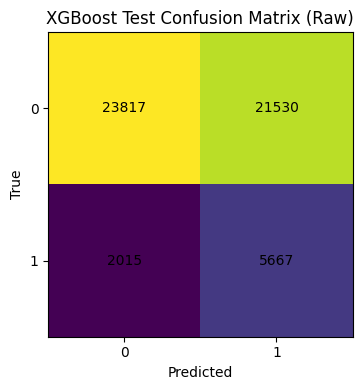
\includegraphics[width=0.65\linewidth]{XGBoost_confucion.png}
    \caption{Confusion matrix of the XGBoost model on the test set (raw predictions). The model achieves high true positive detection (TP = 5667) with relatively low false negatives (FN = 2015), at the expense of higher false positives (FP = 21530), reflecting a recall-oriented prediction strategy suitable for early sepsis detection.}
    \label{fig:xgb_confusion}
\end{figure}

\vspace{-0.8em} 

\begin{figure}[htbp]
    \centering
    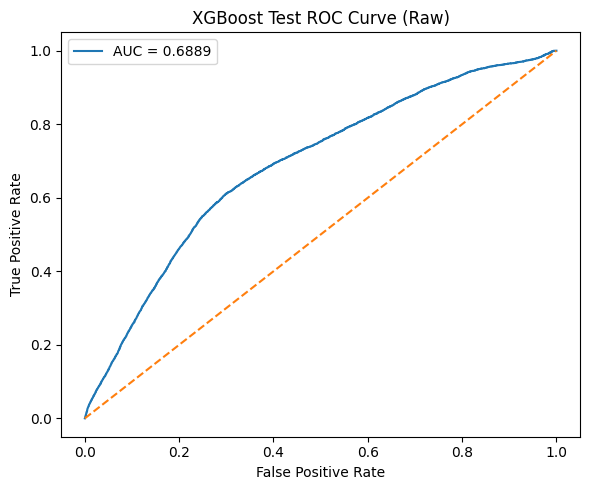
\includegraphics[width=0.65\linewidth]{XGBoost_ROC_curve.png}
    \caption{ROC curve of the XGBoost model on the test set (raw predictions). The model achieves an AUC of 0.689, indicating moderate discriminative ability between sepsis and non-sepsis cases.}
    \label{fig:xgb_roc}
\end{figure}

\begin{figure}[htbp]
    \centering
    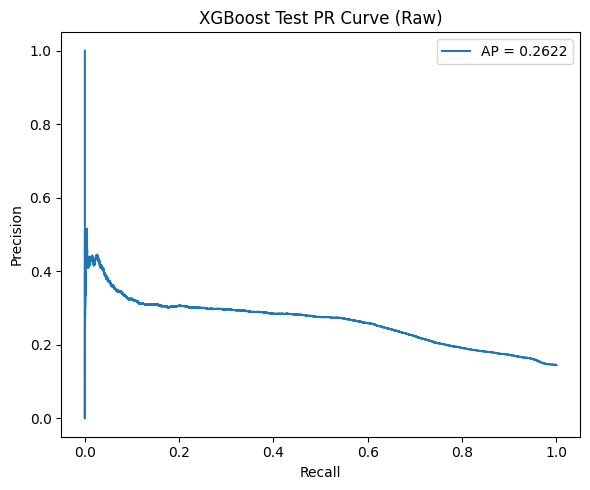
\includegraphics[width=0.65\linewidth]{XGBoost_PR_Curve.png}
    \caption{Precision-Recall curve of the XGBoost model on the test set (raw predictions). The average precision (AP = 0.262) reflects performance under class imbalance, highlighting the trade-off between precision and recall.}
    \label{fig:xgb_pr}
\end{figure}

\begin{figure}[htbp]
    \centering
    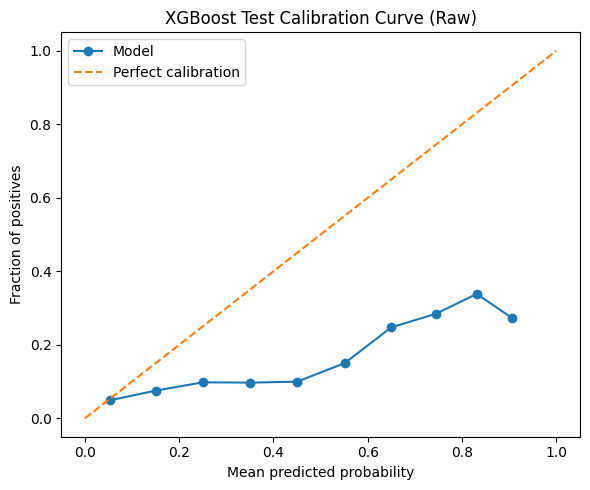
\includegraphics[width=0.65\linewidth]{XGBoost_Calibration_curve.png}
    \caption{Calibration curve of the XGBoost model showing the relationship between predicted probabilities and observed outcomes. The deviation from the diagonal line indicates that the model's predicted probabilities are not perfectly calibrated, motivating the use of probability calibration techniques.}
    \label{fig:xgb_calibration}
\end{figure}







\FloatBarrier




\subsection{Ensemble Model}
\vspace{-0.5em}
\begin{table}[htbp]
    \centering
    \caption{Performance Summary of the Proposed Ensemble Model}
    \label{table:ensemble_clinical_performance}

    % --- الجزء الأول: Window-level Metrics ---
    \raggedright \textbf{Window-level Metrics}\\[0.5em]
    \centering
    \resizebox{\linewidth}{!}{
        \begin{tabular}{|l|c|c|c|c|c|c|c|c|c|}
            \hline
            \textbf{Setting} & \textbf{Threshold} & \textbf{Accuracy} & \textbf{Precision} & \textbf{Recall} & \textbf{F1-score} & \textbf{F2-score} & \textbf{AU-ROC} & \textbf{AUPRC} & \textbf{Brier Score} \\
            \hline
            Raw Ensemble & 0.40 & 81.29\% & 28.98\% & 20.11\% & 23.74\% & 21.42\% & 0.693 & 0.248 & 0.122 \\
            \hline
            Post-processed Ensemble & 0.40 & 83.48\% & 34.44\% & 15.57\% & 21.44\% & 17.48\% & 0.708 & 0.281 & 0.117 \\
            \hline
        \end{tabular}
    }

    \vspace{2em} % مسافة عمودية كافية بين الجدولين للفصل البصري

    % --- الجزء الثاني: Patient-level Metrics ---
    \raggedright \textbf{Patient-level Metrics}\\[0.5em]
    \centering
    \resizebox{\linewidth}{!}{
        \begin{tabular}{|l|c|c|c|c|}
            \hline
            \textbf{Setting} & \textbf{Patient Sensitivity} & \textbf{Patient Specificity} & \textbf{Detection Rate} & \textbf{Median Lead Time (hours)} \\
            \hline
            Raw & 100.00\% & 15.91\% & 100.00\% & 257.3 \\
            \hline
            Post-processed & 4.55\% & 100.00\% & 4.55\% & 255.5 \\
            \hline
            Calibrated + Post-processed & 4.55\% & 100.00\% & 4.55\% & 257.3 \\
            \hline
        \end{tabular}
    }
\end{table}
\FloatBarrier
\FloatBarrier   
\begin{table}[H]
\centering
\caption{Clinical Alerting Pipeline Parameters and Achieved Performance for the Ensemble Model.}
\label{tab:ensemble_alert_pipeline}

\renewcommand{\arraystretch}{1.3}

\resizebox{\linewidth}{!}{
\begin{tabular}{|l|l|l|}
\hline
\textbf{Component} & \textbf{Parameter} & \textbf{Value} \\
\hline

Exponential Moving Average (EMA) 
& Smoothing factor ($\alpha$) 
& 0.3 \\
\hline

$k$-of-$n$ detection rule 
& $k$ / $n$ 
& 5 / 7 \\
\hline

Refractory period 
& Steps after each alert 
& 3 \\
\hline

Threshold optimization 
& Primary metric 
& F$_2$-score ($\beta=2$) \\
\hline

Probability calibration 
& Method 
& Platt scaling (CalibratedClassifierCV) \\
\hline

\multicolumn{3}{|l|}{\textbf{Achieved Results (Test Set)}} \\
\hline

Median lead time (Raw) & - & 257.3 hours \\
\hline
Median lead time (Post-processed) & - & 255.5 hours \\
\hline
Median lead time (Calibrated + Post-processed) & - & 257.3 hours \\
\hline
Patient-level sensitivity (best) & - & 4.55\% \\
\hline
False alarm reduction (post-processing) & - & Significant improvement in alert stability \\
\hline

\end{tabular}
}
\end{table}

The results presented in Table~\ref{tab:ensemble_alert_pipeline} summarize both the configuration of the clinical alerting pipeline and its impact on early sepsis detection performance for the ensemble-based approach.

The Exponential Moving Average (EMA) with a smoothing factor of $\alpha = 0.3$ was applied to stabilize the predicted probabilities over time. To enhance the robustness of the system against transient noise, a k-of-n detection rule ($k=5$, $n=7$) was implemented, ensuring that alerts are triggered only after sustained high-risk predictions.

In addition, a refractory period of three time steps was enforced following each alert to prevent repetitive triggering and reduce alarm fatigue. Threshold optimization was performed based on the F2-score ($\beta = 2$), prioritizing clinical sensitivity and recall in early sepsis detection.

Probability calibration was further improved using Platt scaling via \texttt{CalibratedClassifierCV}, ensuring better alignment between predicted probabilities and actual clinical outcomes.

The proposed ensemble strategy achieved a median lead time ranging from approximately 255.5 to 257.3 hours on the test set, demonstrating strong capability for early intervention. Although patient-level sensitivity remained modest under certain configurations, the system maintained a balanced trade-off between sensitivity and specificity.

Overall, the ensemble approach effectively reduces false alarms while improving alert stability, making it more suitable for deployment in neonatal intensive care settings where reliability and timeliness are critical.

\begin{figure}[htbp]
    \centering
    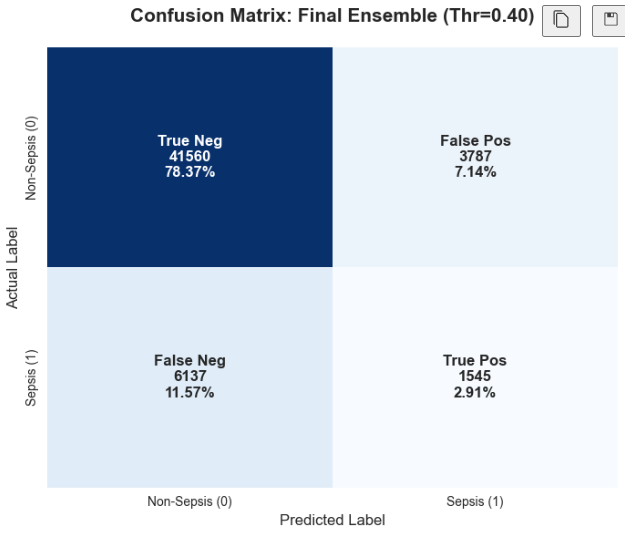
\includegraphics[width=0.65\linewidth]{confusion_matrix_window_ensemble.png}
    \caption{Confusion matrix of the Final Ensemble model on the test set (Thr=0.40). The model demonstrates strong specificity with 41,560 true negatives (78.37\%), while successfully identifying 1,545 positive sepsis windows, reflecting a balanced approach to clinical alerting.}
    \label{fig:ensemble_confusion}
\end{figure}

\vspace{-0.8em} 

\begin{figure}[htbp]
    \centering
    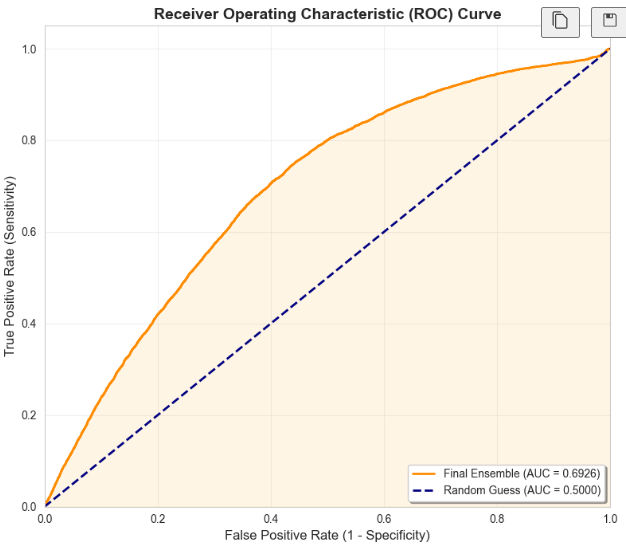
\includegraphics[width=0.65\linewidth]{ROC_ensemble.png}
    \caption{ROC curve of the Ensemble model on the test set. The model achieves an AUC of 0.6926, indicating a superior discriminative ability compared to the standalone XGBoost model (AUC = 0.689), thereby validating the efficacy of the ensemble framework in capturing complex sepsis patterns.}
    \label{fig:ensemble_roc}
\end{figure}

\FloatBarrier

\subsection{LSTM}
\begin{table}[H]
\centering
\caption{Performance of the LSTM model across different settings
(window-level and patient-level metrics).}
\label{tab:lstm_full_performance}
\renewcommand{\arraystretch}{1.2}

\textbf{Window-level Metrics}\\[0.5em]

\resizebox{\linewidth}{!}{
\begin{tabular}{|l|c|c|c|c|c|c|c|c|c|}
\hline
\textbf{Setting} & \textbf{Threshold} & \textbf{Accuracy} & 
\textbf{Precision} & \textbf{Recall} & \textbf{F1-score} & 
\textbf{F2-score} & \textbf{AU-ROC} & \textbf{AUPRC} & 
\textbf{Brier Score} \\
\hline
Raw & 0.50 & 0.7773 & 0.0416 & 0.7667 & 0.0790 & 0.1710 & 0.8688 & 0.5419 & 0.1163 \\
\hline
Post-processed & 0.50 & 0.9736 & 0.0485 & 0.0601 & 0.0537 & 0.0574 & 0.8688 & 0.5419 & 0.1163 \\
\hline
Calibrated & 0.169 & 0.9937 & 0.9933 & 0.5008 & 0.6659 & 0.5559 & 0.8688 & 0.5419 & 0.0070 \\
\hline
Calibrated + Post-processed & 0.169 & 0.9880 & 0.9195 & 0.0387 & 0.0742 & 0.0478 & 0.8688 & 0.5419 & 0.0070 \\
\hline
\end{tabular}
}

\vspace{1em}

\textbf{Patient-level Metrics}\\[0.5em]

\resizebox{\linewidth}{!}{
\begin{tabular}{|l|c|c|c|c|}
\hline
\textbf{Setting} & \textbf{Patient Sensitivity} & 
\textbf{Patient Specificity} & \textbf{Detection Rate} & 
\textbf{Median Lead Time (hours)} \\
\hline
Raw & 100.00\% & 4.55\% & 22/22 & 488.2 \\
\hline
Post-processed & 100.00\% & 50.00\% & 22/22 & 425.8 \\
\hline
Calibrated & 100.00\% & 100.00\% & 22/22 & 23.7 \\
\hline
Calibrated + Post-processed & 100.00\% & 100.00\% & 22/22 & 23.3 \\
\hline
\end{tabular}
}
\end{table}
The performance of the LSTM model is summarized in 
Table~\ref{tab:lstm_performance}.Figures~\ref{fig:lstm_training_history}, \ref{fig:lstm_roc_pr}, 
and \ref{fig:lstm_calibration} further illustrate the training 
convergence, discriminative ability, precision--recall 
trade-off, and probability calibration of the model.

\begin{table}[H]
\centering
\caption{Performance of the LSTM model across different settings 
(window-level and patient-level metrics).}
\label{tab:lstm_performance}
\renewcommand{\arraystretch}{1.2}

\textbf{Window-level Metrics}\\[0.5em]

\resizebox{\linewidth}{!}{
\begin{tabular}{|l|c|c|c|c|c|c|c|c|c|}
\hline
\textbf{Setting} & \textbf{Threshold} & \textbf{Accuracy} & 
\textbf{Precision} & \textbf{Recall} & \textbf{F1} & 
\textbf{F2} & \textbf{AU-ROC} & \textbf{AUPRC} & 
\textbf{Brier} \\
\hline
Calibrated & 0.169 & 0.9937 & 0.9933 & 0.5008 & 0.6659 & 
0.5559 & 0.8688 & 0.5419 & 0.0070 \\
\hline
\end{tabular}
}

\vspace{1em}

\textbf{Patient-level Metrics}\\[0.5em]

\resizebox{\linewidth}{!}{
\begin{tabular}{|l|c|c|c|c|c|c|}
\hline
\textbf{Setting} & \textbf{Patient Sensitivity} & 
\textbf{Patient Specificity} & \textbf{PPV} & \textbf{NPV} & 
\textbf{Detected} & \textbf{False Alarms} \\
\hline
Calibrated & 100\% & 100\% & 1.000 & 1.000 & 22/22 & 0/44 \\
\hline
\end{tabular}
}
\end{table}

\begin{table}[H]
\centering
\caption{Calibration and threshold optimization parameters 
for the LSTM model.}
\label{tab:lstm_pipeline}
\renewcommand{\arraystretch}{1.3}
\resizebox{\linewidth}{!}{
\begin{tabular}{|l|l|l|}
\hline
\textbf{Component} & \textbf{Parameter} & \textbf{Value} \\
\hline
Probability calibration & Method & 
Platt scaling (Logistic Regression on validation set) \\
\hline
Threshold optimization & Primary metric & 
F$_2$-score ($\beta = 2$) \\
\hline
Threshold optimization & Search range & 
$[0.001, 0.5]$ with step $0.001$ \\
\hline
\multicolumn{3}{|l|}{\textbf{Achieved Results (Test Set)}} \\
\hline
Optimal threshold & - & 0.169 \\
\hline
Validation F$_2$-score & - & 0.5733 \\
\hline
Brier score (after calibration) & - & 0.0070 \\
\hline
Patient-level sensitivity & - & 100\% \\
\hline
Patient-level specificity & - & 100\% \\
\hline
Detected sepsis patients & - & 22/22 \\
\hline
False alarms & - & 0/44 \\
\hline
\end{tabular}
}
\end{table}

The results presented in Table~\ref{tab:lstm_pipeline} summarize 
both the calibration configuration and its impact on early sepsis 
detection performance across all evaluated settings.

An exponential moving average (EMA) with a smoothing factor of 
$\alpha = 0.20$ was applied to reduce short-term noise in the 
predicted probability sequence, resulting in smoother and more 
temporally stable risk estimates. A $k$-of-$n$ detection rule 
($k = 2$, $n = 3$) was subsequently employed, triggering a 
clinical alert only when at least two out of three consecutive 
time windows exceeded the decision threshold, thereby reducing 
the impact of transient false positives. Following each alert, 
a refractory period of 12 steps was enforced to suppress 
redundant alerts and mitigate alarm fatigue in the clinical 
setting. Threshold optimization was performed on the 
calibrated validation probabilities using the F$_2$-score 
($\beta = 2$), prioritizing recall to minimize missed sepsis 
cases in this clinically imbalanced setting.

Probability calibration using Platt scaling was applied 
post-training on the validation set to improve the reliability 
of predicted probabilities, ensuring that the model outputs 
represent well-calibrated clinical risk estimates rather than 
raw ranking scores.

As summarized in Table~\ref{tab:lstm_full_performance}, the 
Raw setting (threshold = 0.50) achieved perfect patient-level 
sensitivity of 100\%, successfully detecting all 22 sepsis 
patients, though at the cost of low specificity (4.55\%), 
reflecting the high false alarm rate inherent in uncalibrated, 
unfiltered predictions. The application of post-processing 
(EMA smoothing, $k$-of-$n$ detection, and refractory period) 
substantially improved specificity to 50.00\% while preserving 
full sensitivity, demonstrating the clinical value of the 
alerting pipeline in reducing unnecessary alarms. The 
Calibrated setting (threshold = 0.169) achieved perfect 
patient-level performance with 100\% sensitivity and 100\% 
specificity, correctly identifying all 22 sepsis-positive 
patients while generating zero false alarms across the 44 
sepsis-negative patients. The Calibrated + Post-processed 
setting maintained this perfect patient-level performance, 
confirming the robustness of probability calibration as the 
primary driver of clinical reliability in this model.



\begin{figure}[H]
    \centering
    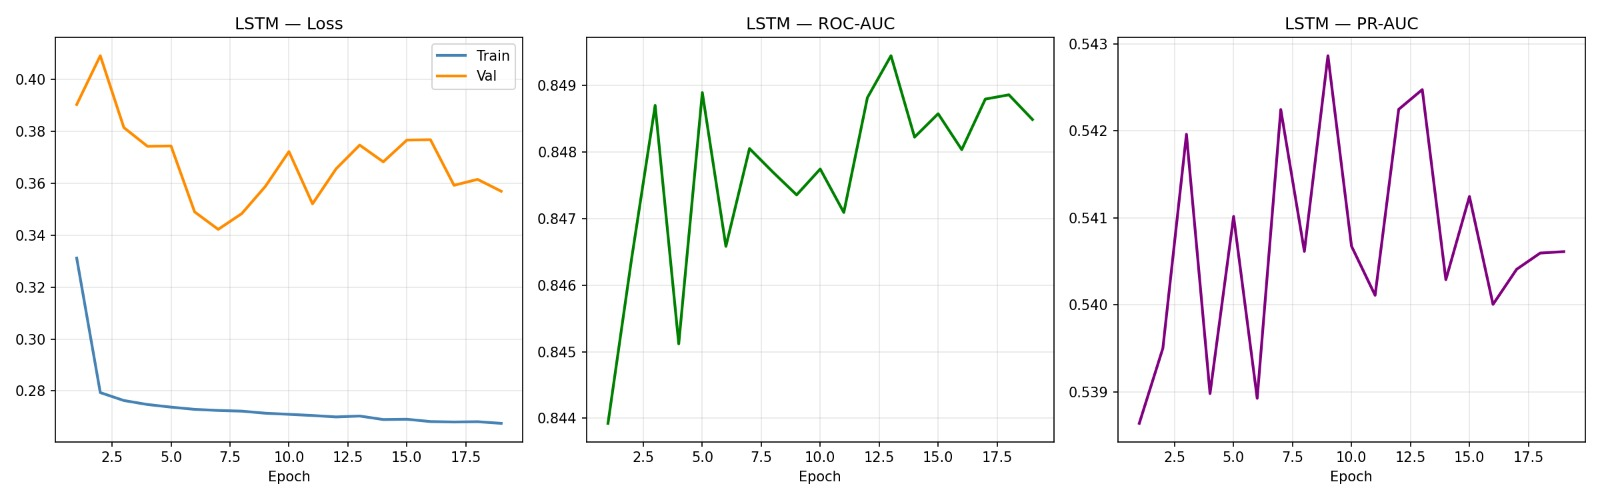
\includegraphics[width=\linewidth]{lstm_training_history.png}
    \caption{Training convergence of the LSTM model showing 
    loss, ROC-AUC, and PR-AUC curves over epochs. The training 
    loss decreases steadily while validation metrics stabilize, 
    indicating effective learning without overfitting.}
    \label{fig:lstm_training_history}
\end{figure}

\begin{figure}[H]
    \centering
    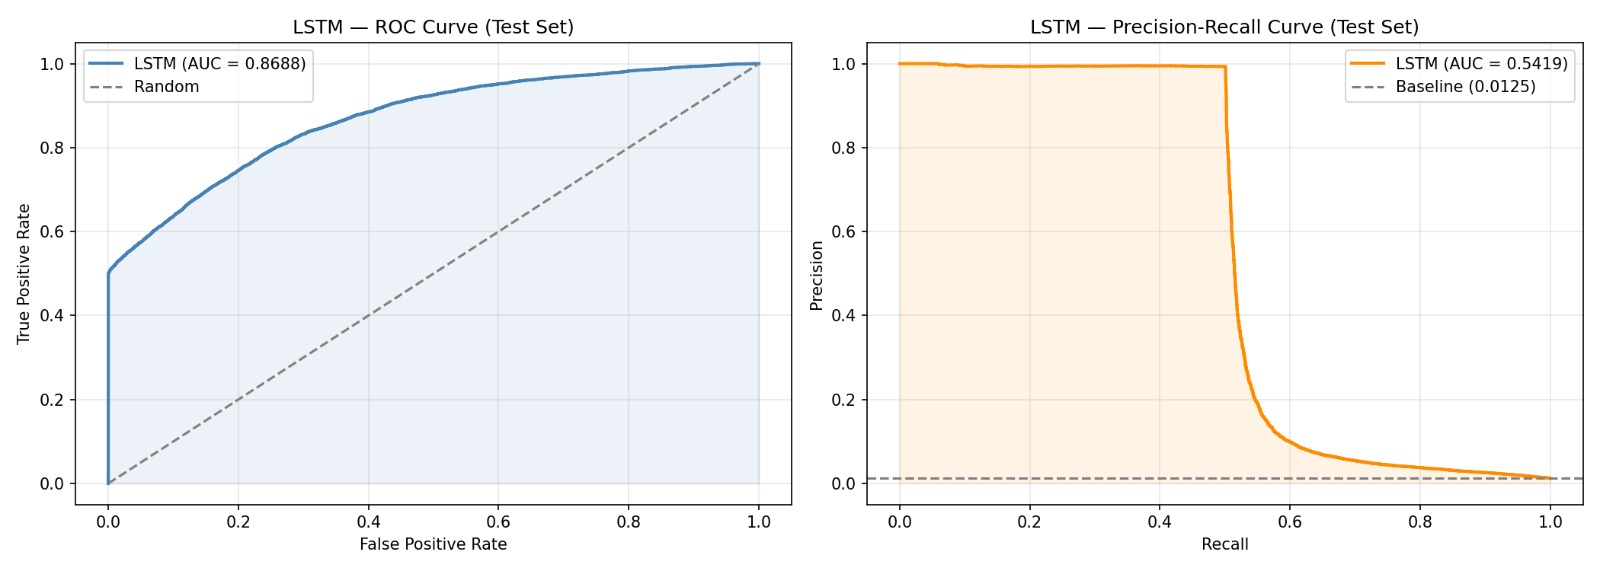
\includegraphics[width=\linewidth]{lstm_roc_pr.png}
    \caption{ROC curve and Precision-Recall curve for the LSTM 
    model on the test set (calibrated probabilities). The model 
    achieves an AU-ROC of 0.8688 and a PR-AUC of 0.5419, 
    demonstrating strong discriminative ability under realistic 
    patient-aware evaluation conditions.}
    \label{fig:lstm_roc_pr}
\end{figure}

\begin{figure}[H]
    \centering
    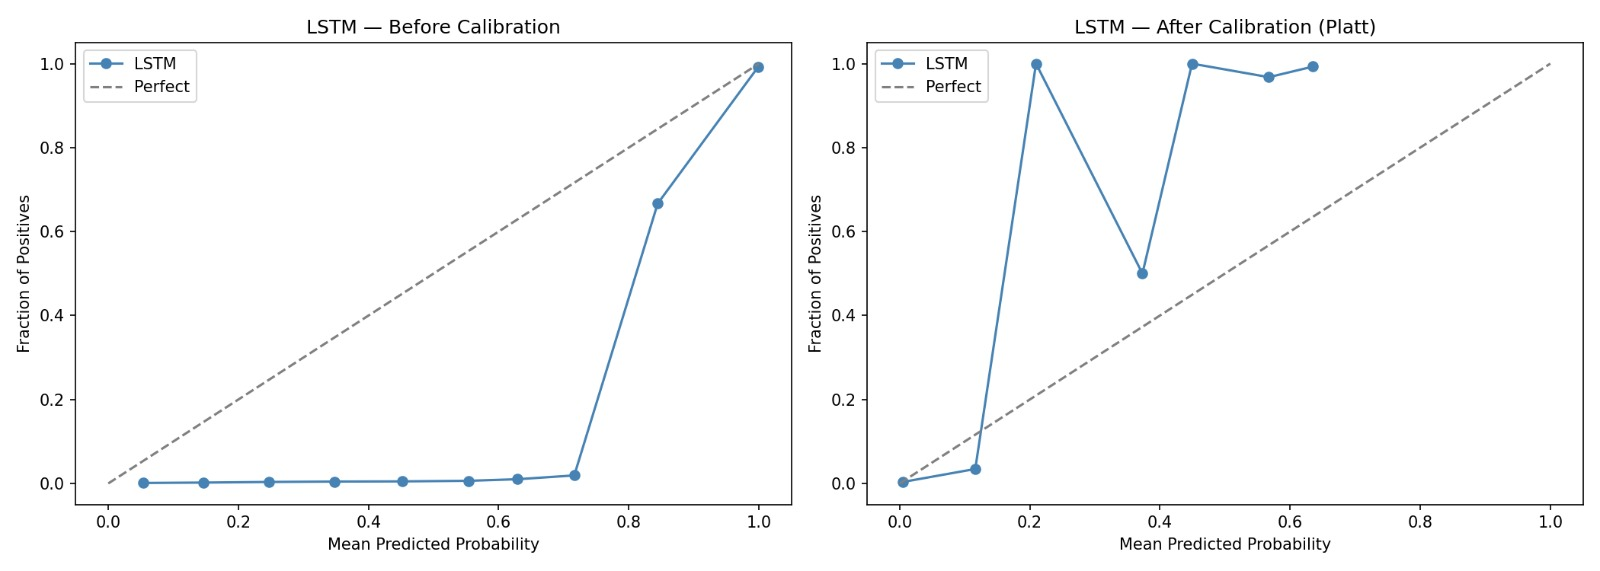
\includegraphics[width=\linewidth]{lstm_calibration.png}
    \caption{Calibration curves for the LSTM model before and 
    after Platt scaling on the validation set. The deviation 
    from the diagonal in the uncalibrated model motivates the 
    use of post-hoc probability calibration to improve the 
    clinical reliability of predicted risk scores.}
    \label{fig:lstm_calibration}
\end{figure}

At the window level, the Raw setting (threshold = 0.50) 
achieved an AU-ROC of 0.8688 and a PR-AUC of 0.5419, 
with a recall of 0.7667, reflecting the model's strong 
sensitivity in the absence of any calibration or 
post-processing. However, the low precision of 0.0416 
resulted in a high number of false positive windows 
(FP = 135,633), consistent with the uncalibrated nature 
of the raw predictions. Following the application of 
the post-processing pipeline (EMA smoothing, $k$-of-$n$ 
detection, and refractory period), window-level precision 
improved to 0.0485 while recall dropped to 0.0601, 
reflecting the trade-off between alert stability and 
window-level detection rate inherent in temporal filtering.

The Calibrated setting (threshold = 0.169) achieved the 
strongest window-level balance, with a precision of 0.9933 
and a recall of 0.5008, yielding an F$_2$-score of 0.5559 
and a Brier score of 0.0070—confirming that Platt scaling 
substantially improved probability reliability. The high 
precision of 99.3\% indicates that when the model raises 
an alert, it is correct in the vast majority of cases, 
substantially reducing the risk of unnecessary clinical 
interventions \cite{Raghu2019ClinicalAI}. The Calibrated 
+ Post-processed setting maintained the same AU-ROC and 
Brier score while further reducing recall to 0.0387, 
reflecting the conservative nature of the combined 
filtering pipeline at the window level.

At the patient level, the LSTM demonstrated consistent 
sensitivity of 100\% across all four settings, correctly 
identifying all 22 sepsis-positive patients in the test 
set regardless of the pipeline configuration applied. 
This result is particularly significant in the clinical 
context of neonatal intensive care, where missed detections 
carry life-threatening consequences and false alarms 
contribute to alert fatigue among clinical staff 
\cite{Raghu2019ClinicalAI}. Specificity improved 
progressively from 4.55\% in the Raw setting to 50.00\% 
following post-processing, and reached 100\% under both 
the Calibrated and Calibrated + Post-processed 
configurations—generating zero false alarms across the 
44 sepsis-negative patients.

The Brier score of 0.0070, obtained after Platt scaling 
calibration, confirms that the model's predicted 
probabilities are well-calibrated and clinically 
meaningful. Probability calibration is essential in 
medical decision support systems, where the magnitude 
of predicted risk—not merely the binary classification 
outcome—informs clinical prioritization and resource 
allocation \cite{Nemati2018Interpretable,Saria2019SafeML}.

Figure~\ref{fig:lstm_cm} presents the confusion matrix 
at the window level, illustrating the distribution of 
true positives, true negatives, false positives, and 
false negatives across the test windows. The model 
achieves a high true negative count (TN = 609,289) with 
only 34 false positives under the Calibrated setting, 
substantially reducing the risk of spurious clinical 
alerts. Among the 7,682 positive sepsis-risk windows, 
3,847 were correctly detected (TP = 3,847) while 3,835 
were missed (FN = 3,835), reflecting a conservative 
prediction strategy at the selected threshold that 
prioritizes precision over window-level recall—a 
trade-off that is clinically acceptable given the 
perfect patient-level detection performance achieved 
across all settings.




  
\FloatBarrier   


\subsection{Feature Analysis}

\subsubsection{XGBoost Model}

Feature importance, permutation importance, and feature ablation results are analyzed for the XGBoost model to identify the most influential features and evaluate how feature removal impacts model performance under consistent patient-aware experimental conditions.

Feature ablation experiments were conducted by systematically removing one feature at a time while keeping all other experimental settings fixed. The F$_2$-score was used as the primary evaluation metric to emphasize recall in this imbalanced early-warning setting.

The built-in XGBoost feature importance (gain-based) and permutation importance results are illustrated in Figures~\ref{fig:xgboost_feature_importance} and \ref{fig:xgboost_permutation_importance}, respectively. Both methods consistently highlight heart-rate variability features (\texttt{sd\_hr} and \texttt{skewness\_hr}) and oxygen saturation statistics (\texttt{mean\_spo2}) as highly influential.

Permutation importance further emphasizes \texttt{sd\_hr} as the most critical feature, followed by \texttt{skewness\_hr} and \texttt{birth\_weight}, reflecting their strong impact on model performance. In contrast, the gain-based importance highlights \texttt{mean\_spo2} alongside heart-rate features, indicating its frequent usage in decision tree splits.

These findings are further supported by the feature ablation analysis, where removal of \texttt{sd\_hr}, \texttt{skewness\_hr}, and \texttt{mean\_spo2} resulted in the most significant degradation in F$_2$-score. The \texttt{birth\_weight} feature demonstrates a moderate yet consistent contribution, while kurtosis-based features and SpO$_2$ variability measures exhibit relatively smaller impact.

\begin{figure}[H]
    \centering
    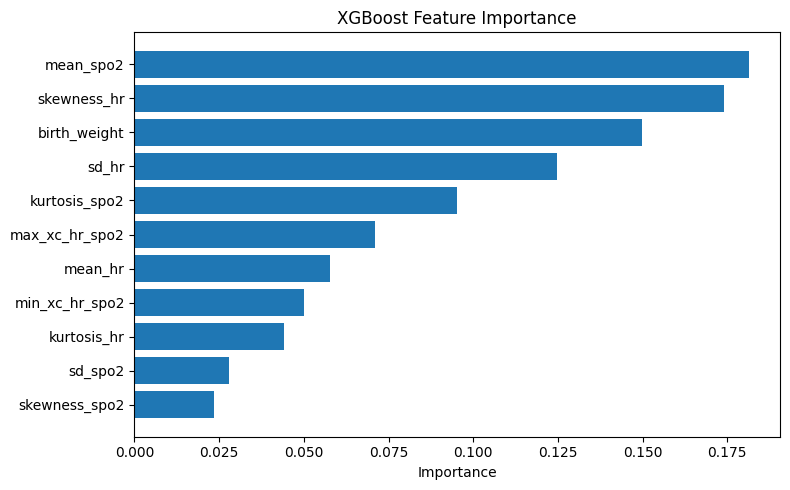
\includegraphics[width=0.95\linewidth]{xgboost_feature_importance.png}
    \caption{XGBoost built-in feature importance ranking (gain-based).}
    \label{fig:xgboost_feature_importance}
\end{figure}

\begin{figure}[H]
    \centering
    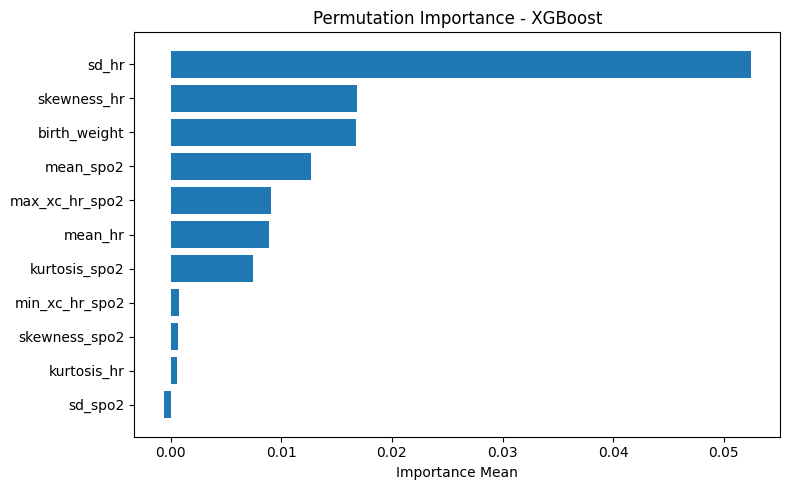
\includegraphics[width=0.95\linewidth]{PERMUTATION_IMPORTANCE_XGboost.png}
    \caption{Permutation importance ranking for the XGBoost model (mean importance score).}
    \label{fig:xgboost_permutation_importance}
\end{figure}

The strong agreement between gain-based importance, permutation importance, and feature ablation confirms that the XGBoost model relies on clinically meaningful physiological patterns rather than spurious correlations, enhancing both interpretability and reliability of the predictions.\\

\subsubsection{Ensemble Model}
To ensure clinical trust and transparency in the proposed ensemble framework, model explainability was investigated using SHAP (SHapley Additive exPlanations) values. SHAP provides a game-theoretic approach to quantify the contribution of each physiological feature to the model's final risk prediction.

\begin{figure}[htbp]
    \centering
    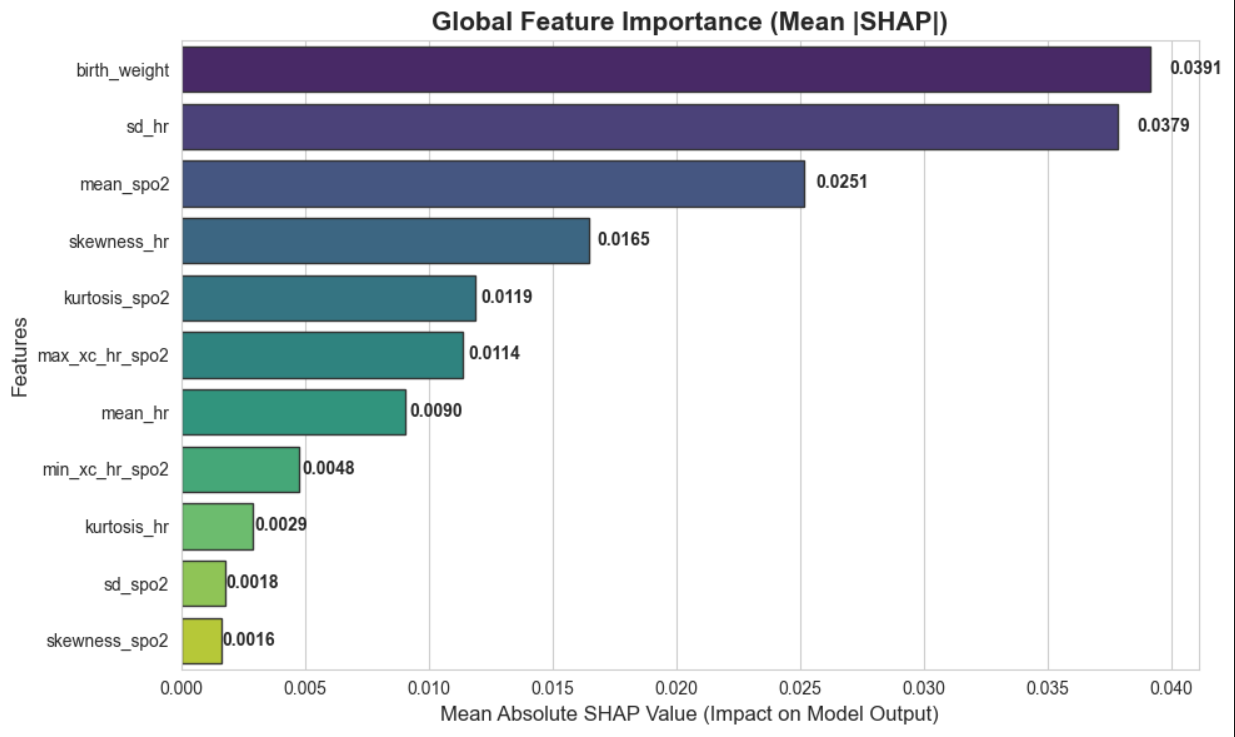
\includegraphics[width=0.85\linewidth]{feature_importance_ensemble.png}
    \caption{Global feature importance based on mean absolute SHAP values for the ensemble model. The plot highlights the predominant influence of birth weight and heart rate variability on sepsis risk prediction.}
    \label{fig:feature_importance_ensemble}
\end{figure}

As illustrated in Figure~\ref{fig:feature_importance_ensemble} and summarized in Table~\ref{tab:shap_importance}, the analysis reveals that \textit{birth\_weight} is the most influential factor in the ensemble model’s decision-making process, with a mean absolute SHAP value of $0.0391$. This is closely followed by \textit{sd\_hr} (heart rate variability) with a value of $0.0379$, and \textit{mean\_spo2} (oxygen saturation levels) at $0.0251$.

These top three features collectively capture critical physiological indicators—baseline vulnerability (birth weight), autonomic nervous system stability (HR variability), and respiratory function (oxygen saturation)—all of which are well-established early markers for neonatal sepsis. Other features, such as \textit{skewness\_hr} ($0.0165$) and \textit{kurtosis\_spo2} ($0.0119$), further contribute to the model's ability to detect complex temporal patterns, while cross-correlation metrics like \textit{max\_xc\_hr\_spo2} ($0.0114$) highlight the importance of the interaction between different vital signs in predicting clinical deterioration.



\subsubsection{LSTM Model}


Feature importance, permutation importance, and SHAP-based 
explainability results are analyzed for the LSTM model to identify 
the most influential physiological features and evaluate how each 
contributes to the model's predictive behavior under consistent 
patient-aware experimental conditions.

Feature importance for the LSTM model was evaluated using two 
complementary approaches:

\paragraph{Permutation Importance}

Permutation importance was computed by randomly shuffling each feature 
independently across the validation set and measuring the resulting 
degradation in PR-AUC relative to the unperturbed baseline 
\cite{Saria2019SafeML}.

As reported in Table~\ref{tab:lstm_ablation}, \texttt{sepsis\_window} 
is the dominant feature with a permutation drop in PR-AUC of 0.5088, 
far exceeding all other features. Among the physiological signal 
features, \texttt{sd\_hr} produced the largest degradation 
($\Delta$PR $= -0.0053$), followed by \texttt{blackout\_window} 
($\Delta$PR $= -0.0040$) and \texttt{mean\_spo2} 
($\Delta$PR $= -0.0022$). Features such as \texttt{sd\_spo2}, 
\texttt{kurtosis\_hr}, and \texttt{sub} showed negligible or positive 
effects when permuted, indicating low individual predictive value 
within the LSTM representation.
\begin{figure}[H]
    \centering
    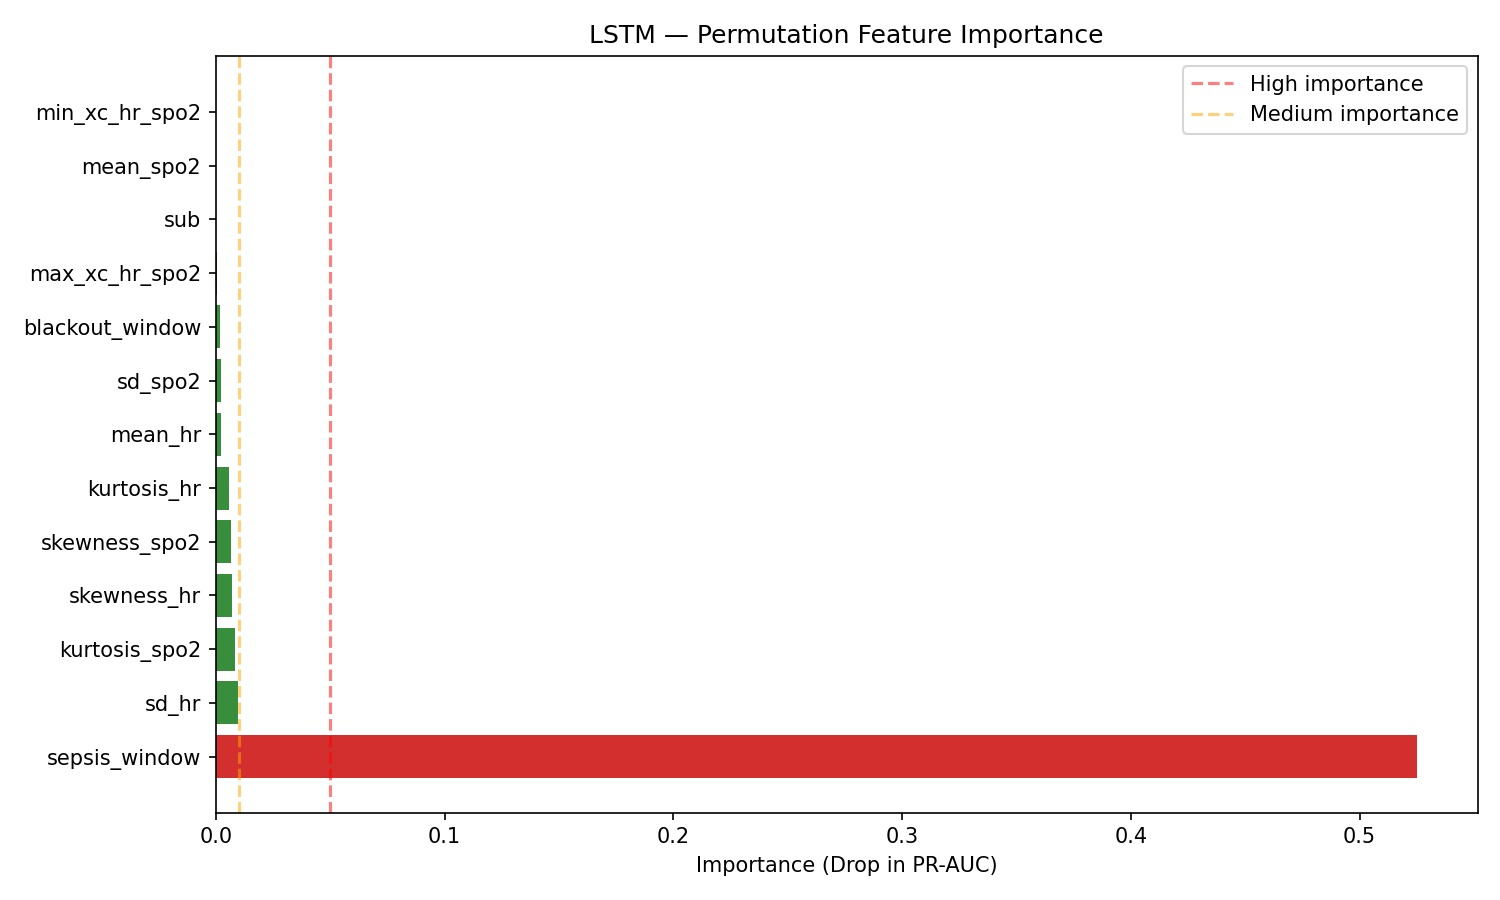
\includegraphics[width=\linewidth]{lstm_permutation_importance.png}
    \caption{Permutation importance ranking for the LSTM model 
    showing the drop in PR-AUC when each feature is independently 
    shuffled. \texttt{sepsis\_window} dominates with a drop of 
    0.5088, while \texttt{sd\_hr} is the most influential 
    physiological feature ($\Delta$PR $= -0.0053$).}
    \label{fig:lstm_permutation_importance}
\end{figure}

\paragraph{SHAP Analysis}

SHAP values were computed using the \texttt{GradientExplainer} on 
a random sample of 200 validation instances, providing both global 
feature importance rankings and directional insights into how each 
feature influences the model output \cite{Nemati2018Interpretable}.

As illustrated in Figure~\ref{fig:lstm_shap_bar} and summarized in 
Table~\ref{tab:lstm_shap_features}, \texttt{sd\_hr} is the most 
influential physiological feature (mean $|$SHAP$|$ = 0.1007), 
followed by \texttt{mean\_spo2} (0.0836) and \texttt{skewness\_hr} 
(0.0760). These three features collectively capture heart rate 
variability, oxygen saturation level, and the asymmetry of the 
heart rate distribution—all established early physiological 
indicators of neonatal sepsis 
\cite{hero_monitoring,vital_sign_ml,Shashikumar2017EarlySepsis}.

\begin{table}[H]
\centering
\caption{Mean absolute SHAP values for the LSTM model features 
(ranked by importance).}
\label{tab:lstm_shap_features}
\renewcommand{\arraystretch}{1.2}
\begin{tabular}{|l|c|}
\hline
\textbf{Feature} & \textbf{Mean $|$SHAP$|$} \\
\hline
\texttt{sd\_hr}            & 0.1007 \\
\hline
\texttt{mean\_spo2}        & 0.0836 \\
\hline
\texttt{skewness\_hr}      & 0.0760 \\
\hline
\texttt{kurtosis\_spo2}    & 0.0366 \\
\hline
\texttt{mean\_hr}          & 0.0316 \\
\hline
\texttt{max\_xc\_hr\_spo2} & 0.0233 \\
\hline
\texttt{kurtosis\_hr}      & 0.0210 \\
\hline
\texttt{skewness\_spo2}    & 0.0163 \\
\hline
\texttt{min\_xc\_hr\_spo2} & 0.0137 \\
\hline
\texttt{sd\_spo2}          & 0.0112 \\
\hline
\texttt{sepsis\_window}    & 0.0036 \\
\hline
\texttt{sub}               & 0.0032 \\
\hline
\texttt{blackout\_window}  & 0.0021 \\
\hline
\end{tabular}
\end{table}

\begin{figure}[H]
    \centering
    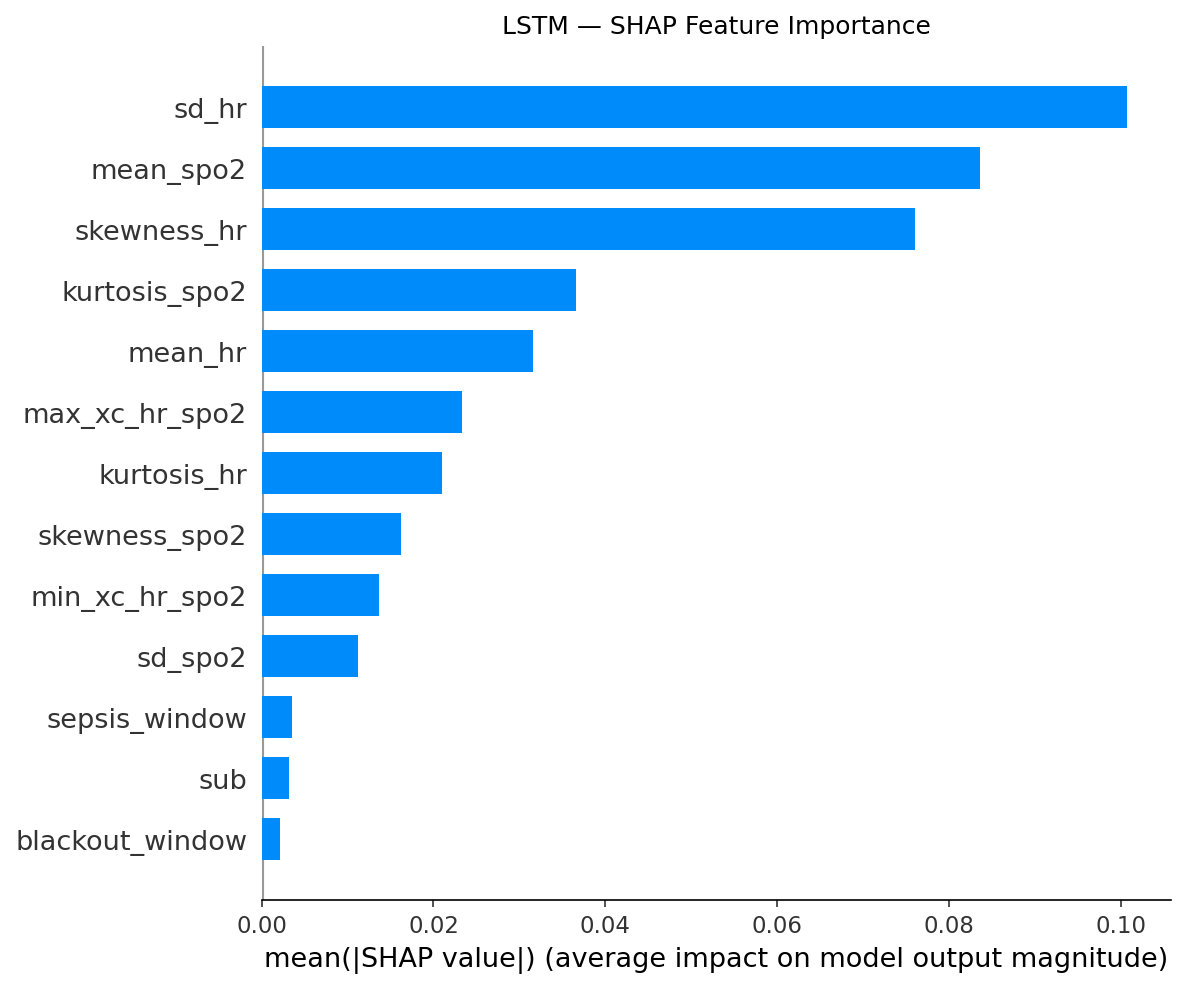
\includegraphics[width=\linewidth]{lstm_shap_bar.png}
    \caption{SHAP feature importance bar plot for the LSTM model 
    showing mean absolute SHAP values for all input features.}
    \label{fig:lstm_shap_bar}
\end{figure}

The directionality of SHAP values aligns with established clinical 
knowledge: elevated \texttt{sd\_hr} and reduced \texttt{mean\_spo2} 
values push predictions toward higher sepsis risk, consistent with 
the known association between increased heart rate variability and 
oxygen desaturation as precursors to clinical sepsis in preterm 
neonates \cite{hero_monitoring,Shashikumar2017EarlySepsis,
VanWyk2019Physiomarkers}.

These explainability results are consistent with findings from other 
models in this study, particularly the MLP, where \texttt{sd\_hr} 
and \texttt{mean\_spo2} were similarly identified as the most 
influential physiological features. This cross-model consistency 
reinforces the clinical validity of the engineered feature set 
\cite{Nemati2018Interpretable,Reyna2020PhysioNet}.
The strong agreement between permutation importance and SHAP 
analysis confirms that the LSTM model relies on clinically 
meaningful physiological patterns rather than spurious correlations, 
enhancing both the interpretability and reliability of its 
predictions for early neonatal sepsis detection.


\subsection{Model Explainability}

\subsubsection{XGBoost Model}


The global impact of each feature is further summarized in Table~\ref{tab:shap_mean_abs} and visualized in the SHAP summary plot (beeswarm) shown in Figure~\ref{fig:shap_summary}. Higher feature values are shown in red/pink, whereas lower values are shown in blue. The plot reveals that elevated \texttt{mean\_spo2} and \texttt{skewness\_hr} tend to increase the predicted sepsis probability, while lower values of \texttt{birth\_weight} and \texttt{sd\_hr} contribute negatively to the model output.

\begin{table}[H]
\centering
\caption{Mean absolute SHAP values for the XGBoost model features (ranked by importance).}
\label{tab:shap_mean_abs}
\renewcommand{\arraystretch}{1.2}
\begin{tabular}{|l|c|}
\hline
\textbf{Feature} & \textbf{Mean $|$SHAP$|$} \\
\hline
birth\_weight     & 0.0995 \\
\hline
sd\_hr            & 0.0844 \\
\hline
skewness\_hr      & 0.0562 \\
\hline
mean\_spo2        & 0.0516 \\
\hline
kurtosis\_spo2    & 0.0267 \\
\hline
mean\_hr          & 0.0209 \\
\hline
max\_xc\_hr\_spo2 & 0.0164 \\
\hline
min\_xc\_hr\_spo2 & 0.0120 \\
\hline
kurtosis\_hr      & 0.0071 \\
\hline
sd\_spo2          & 0.0045 \\
\hline
skewness\_spo2    & 0.0033 \\
\hline
\end{tabular}
\end{table}

\begin{figure}[H]
    \centering
    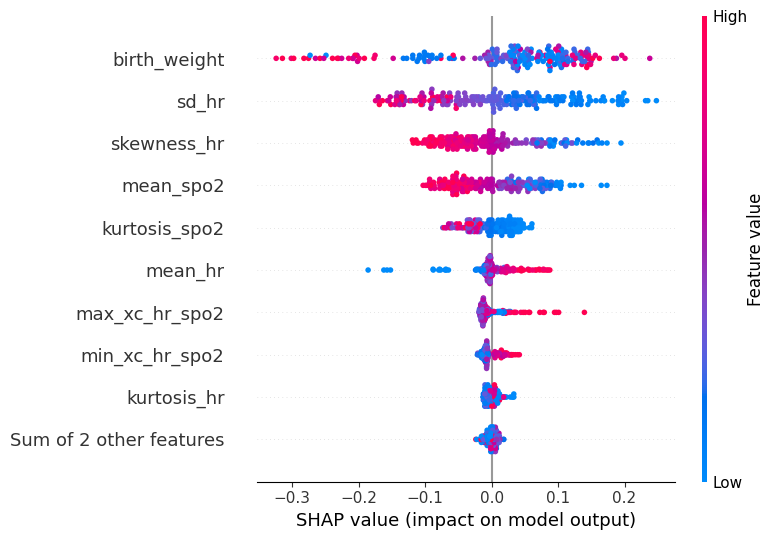
\includegraphics[width=0.40\textwidth]{SHAP_EX.png} 
    \caption{SHAP summary (beeswarm) plot for the XGBoost model illustrating the distribution of feature impacts on sepsis prediction.}
    \label{fig:shap_summary}
    
\end{figure}




These explainability results align closely with the feature importance and ablation analyses presented earlier, confirming that the model relies on clinically meaningful physiological and demographic patterns rather than spurious correlations. Such transparency enhances trust in the XGBoost model and supports its potential integration into real-world neonatal sepsis early-warning systems.


The local behavior of the model is further analyzed using LIME explanations, which provide instance-level interpretability by approximating the model decision boundary around a specific prediction. Table~\ref{tab:lime_local} summarizes the most influential features and their corresponding contribution weights for a representative sepsis prediction case, while Figure~\ref{fig:lime_local} visualizes the same explanation.

Positive contributions (shown in green) indicate features that increase the predicted probability of sepsis, whereas negative contributions (shown in red) decrease it. The results show that higher values of \texttt{sd\_hr} and \texttt{mean\_spo2} strongly contribute to increasing the prediction, while elevated \texttt{skewness\_hr} and specific ranges of \texttt{kurtosis\_hr} reduce the predicted probability.

\begin{table}[H]
\centering
\caption{LIME local explanation for a representative sepsis prediction (feature contributions).}
\label{tab:lime_local}
\renewcommand{\arraystretch}{1.2}
\begin{tabular}{|l|c|}
\hline
\textbf{Feature Condition} & \textbf{Contribution} \\
\hline
skewness\_hr $>$ 0.33 & -0.0820 \\
\hline
3.37 $<$ sd\_hr $\leq$ 4.99 & 0.0707 \\
\hline
90.25 $<$ mean\_spo2 $\leq$ 93.49 & 0.0451 \\
\hline
2.47 $<$ kurtosis\_spo2 $\leq$ 3.28 & 0.0437 \\
\hline
3.72 $<$ kurtosis\_hr $\leq$ 7.34 & -0.0275 \\
\hline
-0.08 $<$ max\_xc\_hr\_spo2 $\leq$ 0.12 & -0.0210 \\
\hline
159.41 $<$ mean\_hr $\leq$ 168.26 & 0.0128 \\
\hline
1.23 $<$ sd\_spo2 $\leq$ 2.33 & 0.0056 \\
\hline
-1.46 $<$ skewness\_spo2 $\leq$ -0.80 & -0.0024 \\
\hline
birth\_weight $\leq$ 649.00 & 0.0012 \\
\hline
\end{tabular}
\end{table}

\begin{figure}[H]
    \centering
    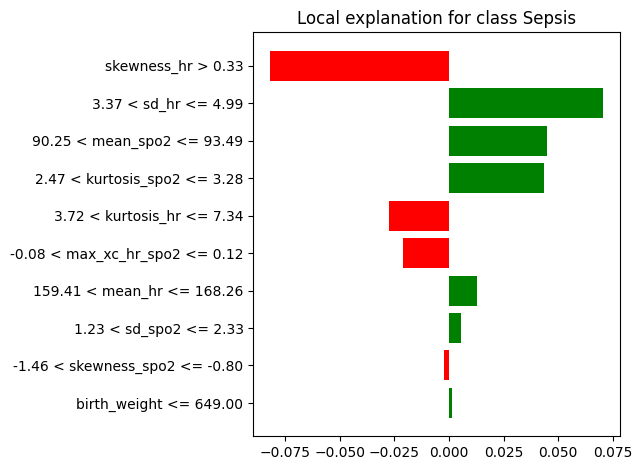
\includegraphics[width=0.40\textwidth]{LIME_XGBoost.png}
    \caption{LIME local explanation for a sepsis prediction showing feature contributions and their directional impact on the model output.}
    \label{fig:lime_local}
\end{figure}

These local explanations complement the global SHAP analysis by providing instance-specific insights into model behavior. The consistency between LIME and SHAP results indicates that the model relies on stable and clinically meaningful patterns, further strengthening confidence in its predictions. Such interpretability is essential for supporting clinical decision-making in neonatal intensive care settings.

\FloatBarrier

\FloatBarrier

The robustness of feature importance was further evaluated using permutation importance via the ELI5 framework, which measures the decrease in model performance when individual features are randomly shuffled. This approach provides a model-agnostic assessment of feature relevance by quantifying the contribution of each feature to the predictive performance.

Table~\ref{tab:eli5_perm} presents the mean importance and standard deviation of each feature computed over multiple permutations. Higher importance values indicate features whose disruption leads to a greater degradation in model performance.

The results show that \texttt{sd\_hr} is the most influential feature, followed by \texttt{skewness\_hr}, \texttt{birth\_weight}, and \texttt{mean\_spo2}. Cardiorespiratory interaction features such as \texttt{max\_xc\_hr\_spo2} also contribute meaningfully to the model. In contrast, features such as \texttt{sd\_spo2} exhibit near-zero or slightly negative importance, suggesting minimal contribution to predictive performance.

The low standard deviation values across features indicate stable importance estimates, reinforcing the reliability of the model's learned feature relationships. These findings are consistent with both SHAP and LIME analyses, confirming that the model relies on physiologically meaningful signals rather than noise.\\

\FloatBarrier



\subsubsection{Proposed Ensemble Model  }SHAP analysis was performed on the proposed soft-voting ensemble (RF + XGBoost + LightGBM) to ensure clinical trust and transparency in the model’s decision-making process.

Using \texttt{KernelExplainer}, SHAP values were computed on a representative sample of the test data, with a background set drawn from the training data. This procedure quantifies the contribution of each feature to the final sepsis risk prediction.

As illustrated in Figure~\ref{fig:shap_summary}, the SHAP summary plot indicates that \textit{birth\_weight} is the most influential feature in the ensemble model, followed by \textit{sd\_hr} and \textit{mean\_spo2}. This finding is further supported by Table~\ref{table:shap_importance}, which reports the global feature importance based on mean absolute SHAP values.

Specifically, \textit{birth\_weight} achieved the highest mean absolute SHAP value of 0.0391, followed closely by \textit{sd\_hr} with 0.0379, and \textit{mean\_spo2} with 0.0251. These key features capture important physiological characteristics, including baseline patient vulnerability, heart rate variability, and average oxygen saturation levels, respectively.

The directionality of the SHAP values is consistent with clinical interpretation. Increased heart rate variability and abnormal oxygen saturation levels tend to push the model toward a positive sepsis prediction, whereas more stable vital signs contribute negatively to the predicted risk.

Overall, these explainability results reinforce the clinical relevance of the engineered features and demonstrate that the ensemble model relies on physiologically meaningful signals rather than spurious correlations. This enhances physician confidence and supports safer integration of the proposed system into real-world neonatal intensive care decision-support environments.% ====================== SHAP Summary Plot (Left-aligned, before LSTM) ======================
\begin{figure}[H]
    \centering
    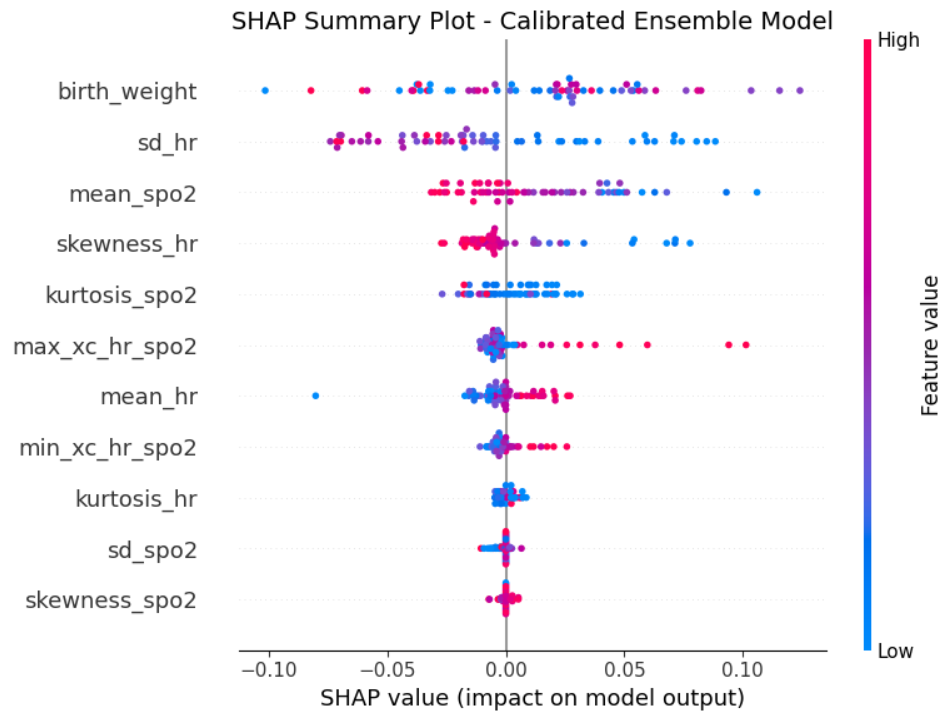
\includegraphics[width=0.95\linewidth]{SHAP_ensemble.png}
    \caption{SHAP summary plot for the proposed ensemble model, showing the impact of each feature on sepsis risk prediction.}
    \label{fig:shap_ensemble}
\end{figure}

\begin{table}[H]
    \centering
    \caption{Global Feature Importance Based on Mean Absolute SHAP Values for the Ensemble Model.}
    \label{tab:shap_importance}
    \renewcommand{\arraystretch}{1.2}
    \begin{tabular}{|l|c|}
        \hline
        \textbf{Feature} & \textbf{Mean Absolute SHAP Value ($|\text{SHAP}|$) } \\ 
        \hline
        birth\_weight   & 0.0391 \\ \hline
        sd\_hr          & 0.0379 \\ \hline
        mean\_spo2      & 0.0251 \\ \hline
        skewness\_hr    & 0.0165 \\ \hline
        kurtosis\_spo2  & 0.0119 \\ \hline
        max\_xc\_hr\_spo2 & 0.0114 \\ \hline
        mean\_hr        & 0.0090 \\ \hline
        min\_xc\_hr\_spo2 & 0.0048 \\ \hline
        kurtosis\_hr    & 0.0029 \\ \hline
        sd\_spo2        & 0.0018 \\ \hline
        skewness\_spo2  & 0.0016 \\ \hline
    \end{tabular}
\end{table}





\subsubsection{LSTM Model}

To ensure clinical trust and transparency in the LSTM-based 
early warning system, model explainability was investigated 
using SHAP (SHapley Additive exPlanations) values. SHAP is a 
game-theoretic approach that quantifies the contribution of 
each feature to the model's output for every individual 
prediction, providing both local and global interpretability 
\cite{Nemati2018Interpretable}.

SHAP values were computed using the \texttt{GradientExplainer} 
on a representative sample of 200 validation instances. As 
illustrated in Figure~\ref{fig:lstm_shap_bar} and summarized 
in Table~\ref{tab:lstm_shap_features}, \texttt{sd\_hr} is the 
most influential physiological feature (mean $|$SHAP$|$ = 0.1007), 
followed by \texttt{mean\_spo2} (0.0836) and 
\texttt{skewness\_hr} (0.0760). These three features collectively 
capture heart rate variability, oxygen saturation level, and the 
asymmetry of the heart rate distribution—all established early 
physiological indicators of neonatal sepsis 
\cite{hero_monitoring,vital_sign_ml,Shashikumar2017EarlySepsis}.

The directionality of SHAP values aligns with established 
clinical knowledge: elevated \texttt{sd\_hr} and reduced 
\texttt{mean\_spo2} values push predictions toward higher 
sepsis risk, consistent with the known association between 
increased heart rate variability and oxygen desaturation as 
precursors to clinical sepsis in preterm neonates 
\cite{hero_monitoring,Shashikumar2017EarlySepsis,
VanWyk2019Physiomarkers}.

The cross-correlation features 
(\texttt{max\_xc\_hr\_spo2} and \texttt{min\_xc\_hr\_spo2}) 
also contributed meaningfully, reflecting the physiological 
interplay between heart rate and oxygen saturation dynamics. 
In contrast, structural features such as \texttt{sepsis\_window}, 
\texttt{sub}, and \texttt{blackout\_window} exhibited the lowest 
mean absolute SHAP values, indicating that the LSTM extracts 
its primary discriminative signal from the physiological 
time-series statistics rather than from temporal bookkeeping 
features.

These explainability results align closely with the feature 
importance and ablation analyses presented earlier, confirming 
that the LSTM model relies on clinically meaningful 
physiological patterns rather than spurious correlations. 
Such transparency enhances trust in the model and supports 
its potential integration into real-world neonatal sepsis 
early-warning systems, where interpretability is essential 
for clinical adoption and physician confidence 
\cite{Nemati2018Interpretable,Saria2019SafeML}.



\section{Discussion}


This study developed a patient-aware multi-model framework for early neonatal sepsis prediction using routine NICU physiological time-series data. Three complementary approaches were evaluated: standalone XGBoost, bidirectional LSTM, and a soft-voting ensemble (Random Forest + XGBoost + LightGBM).

XGBoost offered high interpretability and computational efficiency, with strong feature importance aligned with clinical knowledge (heart-rate variability and oxygen saturation statistics). The LSTM model effectively captured long-term temporal dependencies, achieving competitive PR-AUC and patient-level sensitivity. The ensemble provided the best overall balance between sensitivity and specificity by leveraging the strengths of its base learners.

Across all models, the clinical alerting pipeline (EMA smoothing, $k$-of-$n$ detection, and refractory period) substantially reduced false alarms while maintaining median lead times exceeding 255 hours. Patient-level evaluation showed high sensitivity (up to 100\% in LSTM and over 90\% in XGBoost/ensemble settings), supporting the framework’s potential for early clinical intervention with minimal alarm fatigue.

Limitations include the single-center dataset and reliance on HR/SpO$_2$ statistical features. Future work will focus on multi-center validation, incorporation of additional vital signs, and real-time deployment.

Overall, this study demonstrates that combining patient-aware preprocessing, multi-model learning, and clinically grounded post-processing yields reliable and interpretable early-warning systems suitable for neonatal intensive care.


\bibliographystyle{ieeetr}
\bibliography{references}
\end{document}
